
%%%%%%%%%%%%%%%%%%%%%%% file template.tex %%%%%%%%%%%%%%%%%%%%%%%%%
%
% This is a general template file for the LaTeX package SVJour3
% for Springer journals.          Springer Heidelberg 2010/09/16
%
% Copy it to a new file with a new name and use it as the basis
% for your article. Delete % signs as needed.
%
% This template includes a few options for different layouts and
% content for various journals. Please consult a previous issue of
% your journal as needed.
%
%%%%%%%%%%%%%%%%%%%%%%%%%%%%%%%%%%%%%%%%%%%%%%%%%%%%%%%%%%%%%%%%%%%
%
% First comes an example EPS file -- just ignore it and
% proceed on the \documentclass line
% your LaTeX will extract the file if required
\begin{filecontents*}{example.eps}
%!PS-Adobe-3.0 EPSF-3.0
%%BoundingBox: 19 19 221 221
%%CreationDate: Mon Sep 29 1997
%%Creator: programmed by hand (JK)
%%EndComments
gsave
newpath
  20 20 moveto
  20 220 lineto
  220 220 lineto
  220 20 lineto
closepath
2 setlinewidth
gsave
  .4 setgray fill
grestore
stroke
grestore
\end{filecontents*}
%
\RequirePackage{fix-cm}
%
\documentclass[twocolumn]{svjour3}                     % onecolumn (standard format)
%\documentclass[smallcondensed]{svjour3}     % onecolumn (ditto)
%\documentclass[smallextended]{svjour3}       % onecolumn (second format)
%\documentclass[twocolumn]{svjour3}          % twocolumn
%
\smartqed  % flush right qed marks, e.g. at end of proof


%
% \usepackage{mathptmx}      % use Times fonts if available on your TeX system
%
% insert here the call for the packages your document requires
%\usepackage{latexsym}
% etc.
\usepackage{natbib}
\usepackage{graphicx}
\usepackage{citeref}
\usepackage{epsfig} % for postscript graphics files
\usepackage{mathptmx} % assumes new font selection scheme installed
\usepackage{times} % assumes new font selection scheme installed
\usepackage[cmex10]{amsmath} % assumes amsmath package installed
\usepackage{textcomp} %helps with math symbols
\usepackage{caption}
\usepackage{subcaption}
\usepackage{subfig}
\usepackage{amssymb}  % assumes amsmath package installed
\usepackage{multirow}
\usepackage{array}
\usepackage{mdwtab}
\usepackage{bigstrut}
% please place your own definitions here and don't use \def but
% \newcommand{}{}
%
% Insert the name of "your journal" with
 \journalname{Autonomous Robots}
%
\begin{document}

\title{Analysis of Adaptive Sampling Techniques for Underwater Vehicles}%\thanks{Grants or other notes 
%about the article that should go on the front page should be
%placed here. General acknowledgments should be placed at the end of the article.}
%}

%\subtitle{Do you have a subtitle?\\ If so, write it here}

%\titlerunning{Short form of title}        % if too long for running head

\author{Andres~Mora \and Colin~Ho \and Srikanth~Saripalli}

%\authorrunning{Short form of author list} % if too long for running head

\institute{A. Mora, C. Ho, and S. Saripalli \at
              School of Earth and Space Exploration, Arizona University,
550 E. Tyler Mall, Tempe, Arizona, 85287 \\
              Tel.: +1-480-823-5555\\
              Fax: +1-23-45-678910\\
              \email{\{amoravar, colin.ho, srikanth.saripalli\}@asu.edu}
}

\date{Received: date / Accepted: date}
% The correct dates will be entered by the editor


\maketitle

\begin{abstract}
A critical problem in planning sampling paths for autonomous underwater vehicles is correctly balancing two issues.
First, obtaining an accurate scalar field estimation and second, efficiently utilizing the stored energy capacity of the sampling vehicle. 
Adaptive sampling approaches can only provide solutions when real-time and a priori environmental data is available. 
In this paper we present an analysis of adaptive sampling methodologies for autonomous underwater vehicles.
In particular, we analyze various sampling path strategies including systematic and stratified random patterns within a wide range of sampling densities and their impact in the energy consumption of the vehicle through a cost-evaluation function.
Our study demonstrates that a systematic spiral sampling path strategy is optimal for high-variance scalar fields for all sampling densities and low-variance scalar fields when sampling is sparse. 
In addition, our results show that the random spiral sampling path strategy is found to be optimal for low-variance scalar fields when sampling is dense.

\keywords{Experimental \and Optimal \and Adaptive Sampling \and Autonomous Underwater Vehicles \and kriging}
% \PACS{PACS code1 \and PACS code2 \and more}
% \subclass{MSC code1 \and MSC code2 \and more}
\end{abstract}

\section{Introduction}
\label{intro}
{A}{utonomous} underwater vehicles (AUV) are mobile robotic platforms that are utilized for environmental sampling, sensing and are capable of operating in a multitude of underwater aquatic environments \citep{forrest:investigation}.
In research they are commonly used to carry hydrological, geophysical, and/or biological sensor payloads.
These payloads are typically used to gather remote and in-situ data to aid the study of open and closed aquatic bodies \citep{stoker:exploration}, \citep{german:hydro}.

\begin{figure}[htp]
	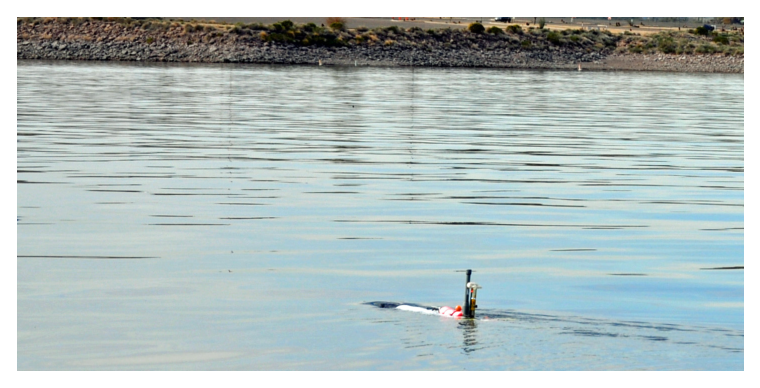
\includegraphics[width=\columnwidth, scale= 0.6]{figs/iverAtPleasant} 
	\caption{Modified OceanServer IVER2 AUV at Lake Pleasant.}
	\label{fig:iverAtPleasant}
\end{figure}

An autonomous underwater vehicle is generally described as being capable of operation without any human controller; thus it must be able to traverse the aquatic environment on a desired path through autonomous navigation and control \citep{kumagai:newAUV}. 
The autonomous underwater vehicle used to collect the data analyzed in this paper is shown in Figure \ref{fig:iverAtPleasant}. 	

The goal of environmental sampling and sensing is to generate an accurate estimate of the underlying scalar field(s) over an area of interest. 
Generally, an estimate is generated by interpolating the sensing data collected over the area being studied. 
In the case of aquatic environments, a mobile vehicle can be introduced for it to autonomously collect the necessary sensing data. 

However a number of questions need to be answered before deciding on a strategy to gather these data.
When using an AUV as sensing platform its range is limited by the amount of stored energy. 
The problem of environmental sensing then becomes determining how one obtains an accurate estimation of the scalar field of interest while being constrained by the amount of stored energy the vehicle can utilize in order to sample the scalar field.
Moreover, what sampling pattern should be used to accurately determine the underlying scalar field?
How and under which conditions shall a particular sampling pattern be performed?
What are the parameters that constraint such selection?
Furthermore, is it possible to estimate the values of the underlying scalar field of an area in the future based on previous measurements taken from nearby locations?

The purpose of this paper is to experimentally evaluate sampling strategies based upon estimation accuracy and energy consumption.
The paper also shows the result of a scalar field estimation of a given area based on the measurements previously gathered at a different nearby location.
 
The evaluation of the sampling strategies is conducted with a cost-evaluation function that considers multiple parameters (such as the AUV's power consumption), and can assign priorities to each factor. 
Incorporating a dynamical model of the AUV rather than a simplified energy consumption model to the proposed cost-evaluation function, allows to relax the assumptions made of its movement and provides a better approximation of the vehicle's power consumption performance during a given sampling path.

\begin{figure}[tp]
	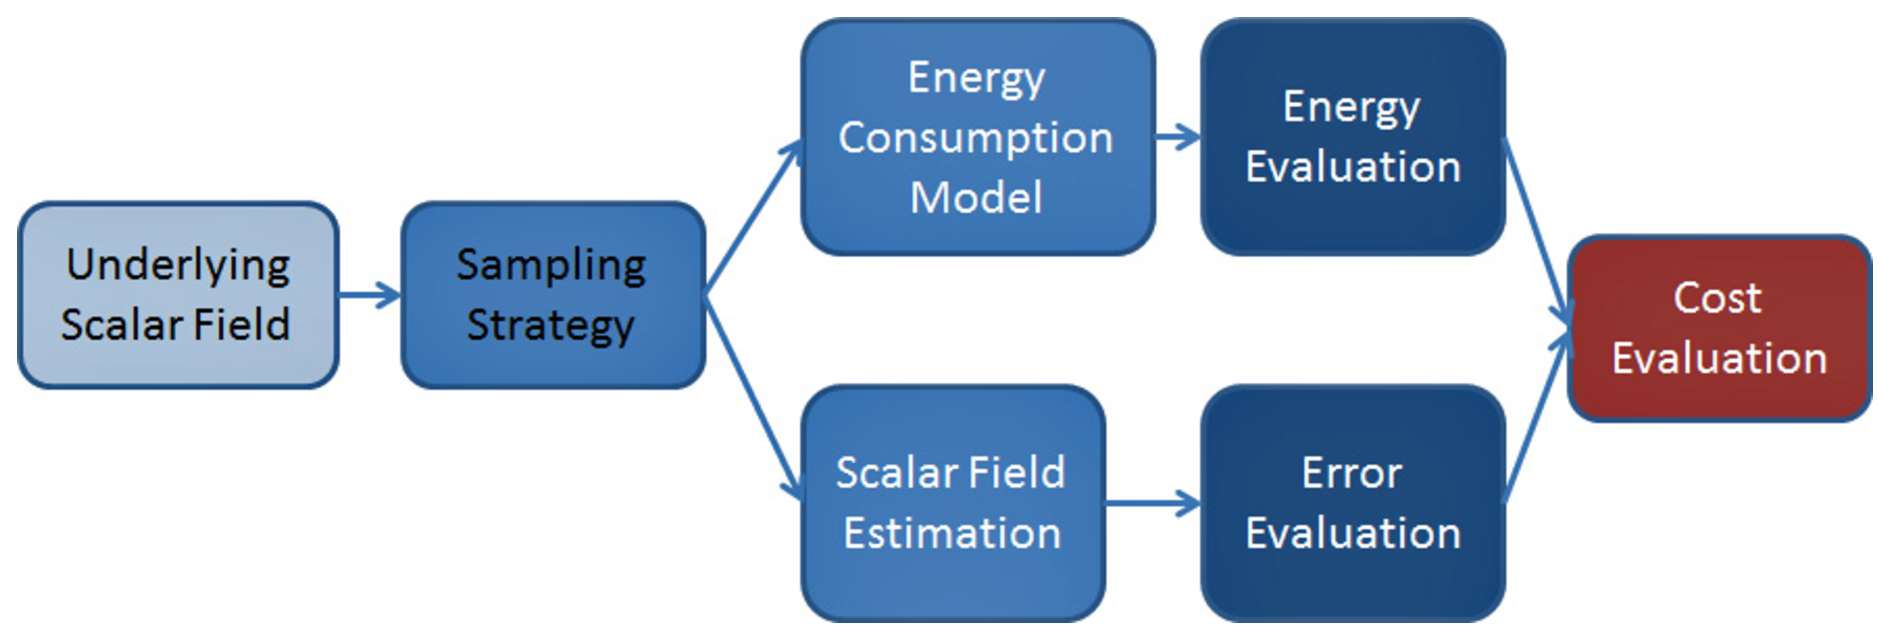
\includegraphics[width=\columnwidth, scale= 1.0]{figs/paperFlowExplanation}
	\caption{Experiment and analysis general description.}
	\label{fig:paperFlowExplanation}
\end{figure}

The evaluation takes into account real world and simulated isotropic, anisotropic scalar fields, as well as varying sampling densities to determine which sampling strategy is optimal for different scalar field types, for a range of sampling densities. 
The sampling path strategies evaluated in this study were systematic and stratified random sampling distributions with spiral and lawn mower sampling paths.

The research presented in this paper follows the flow presented in Figure \ref{fig:paperFlowExplanation}.
After having gathering in-situ data, we observe the underlying scalar field present at data sampling area.
Based on the data sets obtained, we produce different sampling strategies over the underlying scalar field.
At this point we evaluate two important factors: the energy consumption of the vehicle and the error in the estimation of a scalar field obtained from the data set.
Finally, we determine the optimal sampling strategy for a set of underlying scalar fields from the sampling patterns we studied.
For this process we analyze the interaction of multiple factors affecting the vehicle by applying a cost-evaluation function. 

We demonstrate with the results of the cost-evaluation function that the systematic spiral sampling path strategy best optimizes the energy consumption with the scalar reconstruction error compared to the other sampling path strategies evaluated. 
Additionally, it is found that the systematic spiral path consumes the least amount of energy out of the sampling path strategies evaluated.

%%%%%%%%%%%%%%%%%%%%%%%%%%%%%%%%%%%%%%%%%%%%%
\section{Related Work}
\label{relWork}

In the fields of robotics, hydrology, geology, and geostatistical sciences, optimal sample collection and path planning are an active area of research \citep{mcbratney:exploration}. 
There is much prior and current work ongoing in the domain of path planning and sampling optimization for autonomous vehicles. 
For example, adaptive sampling algorithms have been developed that can direct the path of single or multiple autonomous underwater vehicles in towards locations of high probable data yield \citep{popa:adaptive}, and can be used in conjunction with existing sensor networks \citep{zhang:adaptive}. 
Additionally, energy optimal paths can be computed based upon known and sensed external variables such as ocean currents \citep{witt:go}-\citep{smith:autonomous}, and static or dynamic obstacles \citep{caldwell:reconfiguring}.

Adaptive sampling is an emerging methodology that aims to balance the trade-off between establishing the optimal dimension of a sampling grid, energy consumed by the AUV and the total duration of the mission.
The autonomy of this procedure is accomplished by the addition of algorithms that incorporate online, real-time taken measurements of the environment to correct and consequently, improve the sampling made by the AUV.

Cruz et. al \citep{cruz:thermoclines} developed an algorithm to detect and track thermoclines using a vertical, gradient-based model first proposed by Haeger \citep{haeger:vertGradModel}. 
Cruz's work achieved tracking in low resolution temperature environments, with separations of aproximately $1$ \textcelsius and maximum gradients in the range of $0.2-0.3\,^{\circ}\mathrm{C}/m$. 
However this work does not detail the energy consumption of the vehicle throughout the mission nor how did the algorithm affect the length of the mission. 

Work has also been done to study the advantages and disadvantages of multiple AUVs collaborating towards adaptive sampling of bodies of water.
Popa \citep{popa:adaptive} proposed a platform that uses multiple, collaborating AUVs to study the classic robotics problem of localizing multiple AUV but with the application of estimating a distributed field variable.
In this work, the authors model the energy consumption as a damping coefficient as part of their potential fields.
Chen et. al \citep{chen:adaptive} on the other hand, uses an approach based on a lawn-mower sampling pattern which consists of two phases. 
After having completely surveyed the field of interest in phase I, the authors sample the region again while minimizing the maximum reconstruction error and then resample the region while minimizing the energy consumption. 
They further show this approach outperforms the Random Compressive Sensing (RCS) and Deterministic Compressive Sensing (DCS) presented by \citep{donoho:compressed} and \cite{devore:deterministic}, respectively.
In our proposed methodology, we have determined which paths are optimal for underlying scalar fields based on either simulation-generated or in-situ acquired data.

%%%%%%%%%%%%%%%%%%%%%%%%%%%%%%%%%%%%%%%%%%%%%
\section{Experimental Design Principles}
\label{principles}

Previous work on autonomous adaptive sampling has focused on planning schemes that require either a priori knowledge of the environment, or real time in-situ sensing and data feedback. 
However in real world AUV deployments, the sampling strategies and paths that are chosen are often simple lawnmower patterns that may not be optimal for the situation they are utilized in  \citep{forrest:investigation}, \citep{stoker:exploration}. Thus the fundamental question that is raised is which sampling path strategy the optimal strategy for off-line AUV deployments, and for what type of underlying scalar field are they optimal for?

From an experimental perspective, one is often interested in obtaining a sampling strategy that is optimal; particularly in maximizing coverage area while minimizing time or distance to better use the limited energy on-board the vehicle.
In order to answer the question of sampling path strategy optimality, the problem must be evaluated from an experimental field scientist's data sampling perspective. 
Optimality for a field scientist would be defined as maximizing data return, while minimizing the estimation error of the data from the underlying scalar field being sampled. 
Sampling path strategies must then be evaluated for a variety of underlying scalar field data types that would be representative of real world data. 
Thus, an means of comparatively evaluating various sampling path strategies must be created and applied to various sampling path strategies across a wide range of scalar field data types. 
In this evaluation, a multi-parameter cost evaluation function was created such that optimality can be defined by the specific needs of the field scientist. 
However before any evaluation can be conducted, real world data sets must be collected to form the basis on which the evaluations can be held. 

%%%%%%%%%%%%%%%%%%%%%%%%%%%%%%%%%%%%%%%%%%%%%
\section{Experimental Framework}
\label{expFramework}
The real world data sets were collected with an AUV platform specially outfitted with the instrumentation necessary to conduct a comprehensive characterization of underlying scalar fields.
 
\subsection{AUV Platform: IVER}
Our AUV platform is based on the MIT-developed aquatic robotic platform called ``IVER2 Ocean Server''~\citep{iver2:internet}.
This robotic platform has a diameter of 14.7 cm, a length of 127 cm, it weights 20 kg approximately, and it has a maximum operation depth of 100 m. 

It has several navigational and environmental sensors onboard: GPS, CTD unit, sonar and our group has modified it such that its body can accomodate several cameras that are used during mapping tasks.
The platform is powered by a set of 95 WHr, 14.4 V, 6.6 Ah Li-Ion smart battery packs.
It has 4 independent fins making it possible to control the robot's yaw, pitch and allowing for an active roll correction. 
Its propulsion is based on a direct drive DC brushless motor. 

It also has two main computers on-board (based on an Intel ATOM 1.6 GHz) that are in charge of navigation and mapping tasks.
The robot can be given commands remotely through its WiFi access point within a 1 km range; in the event of an emergency the vehicle can be then commanded to stop its mission and go back to safety.

The robotic platform and its instrumentation payload used in this research are shown in Figure \ref{fig:iver}-\ref{fig:ysiSonde}. 

\begin{figure}
\centering
	\begin{subfigure}[t]{0.485\textwidth}
    	\centering
        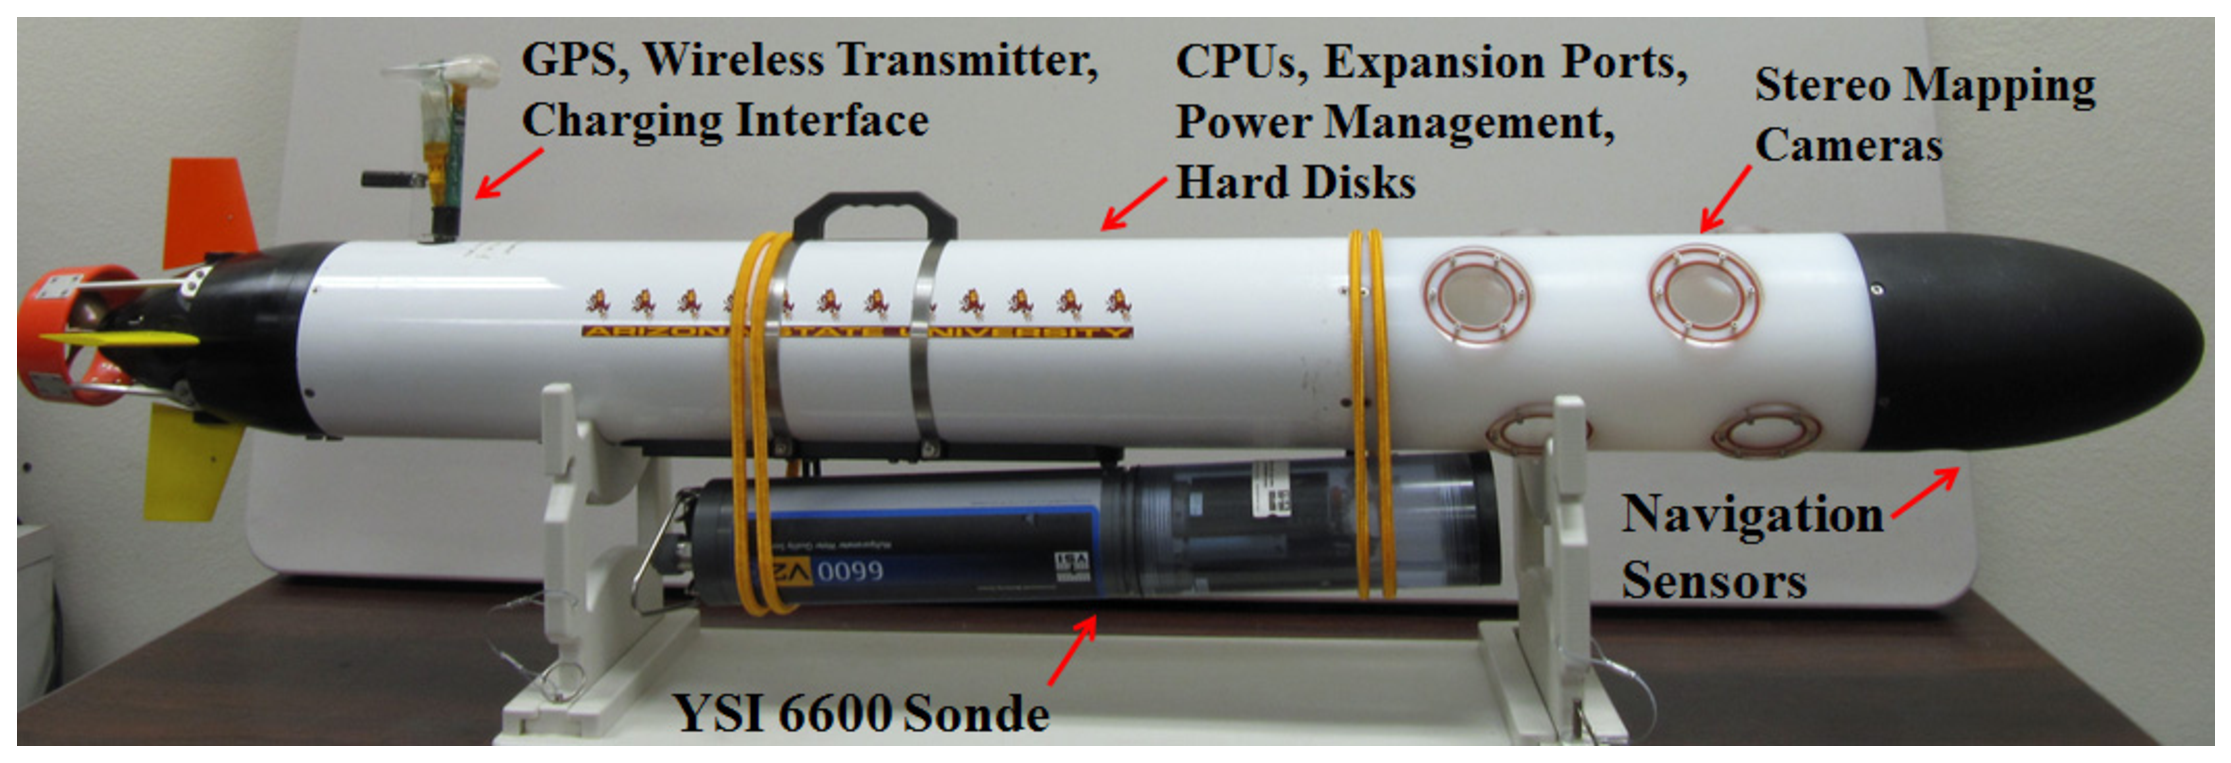
\includegraphics[width=\columnwidth, scale= 1.0]{figs/iverDescription1} %width=\columnwidth, scale= 1.0
        \caption{IVER: AUV testbed used during the autonomous sampling experiments presented in this paper.}
        \label{fig:iver}
     \end{subfigure}
     
     \vspace{0.5cm}
     
     \begin{subfigure}[b]{0.30\textwidth}
    	\centering
        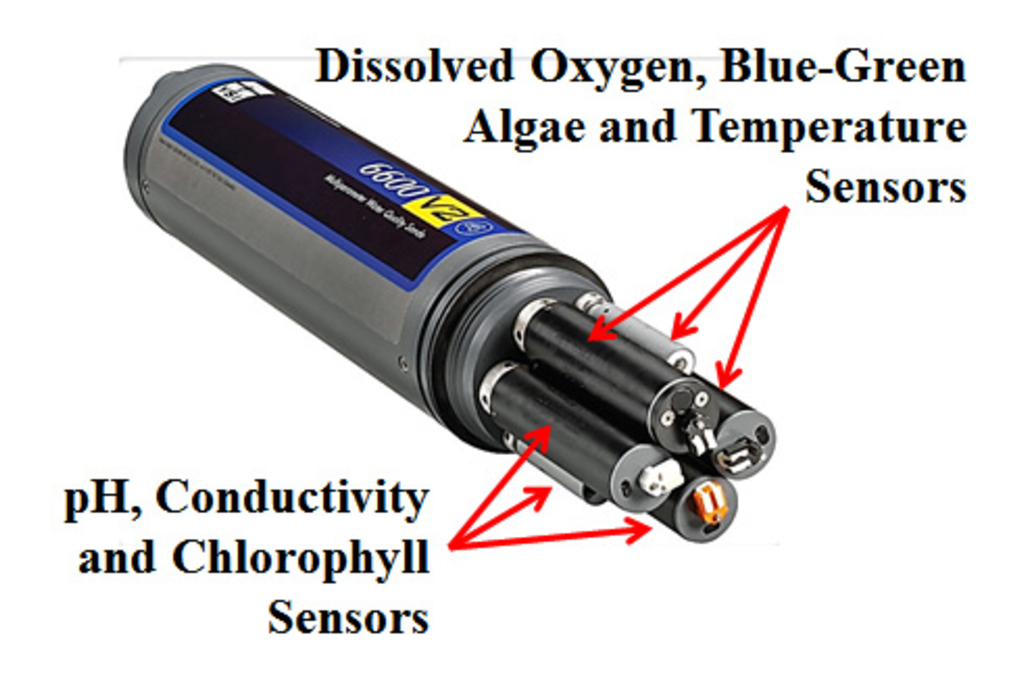
\includegraphics[width=\columnwidth, scale= 0.35]{figs/iverSonde1} %width=\columnwidth, scale= 1.0
        \caption{YSI Sonde.}
        \label{fig:ysiSonde}
     \end{subfigure}
\caption{Experimental Test-bed used during the autonomous sampling presented in this paper.}
\label{fig:testBed}
\end{figure}

The instrumentation payload carried by our robotic platform was based on the YSI6600 sonde. 
This sonde measures temperature, turbidity, blue green algae (BGA), pH, dissolved oxygen and chlorophyll simultaneously. Standard measurement ranges for each of its sensors are summarized in Table \ref{tab:ysiSonde}. 

The sonde has a diameter of 8.9 cm, a length of 54.9 cm, and a weight of 3.18 kg. It is powered by 8C-size alkaline batteries, it can operate between $-5$ \textcelsius to $+50$ \textcelsius.

\begin{table}
  \begin{center}
  	\caption{Characteristics of the Instruments on the YSI Sonde}
  	\label{tab:ysiSonde}
    \begin{tabular}{|m{2.2cm}|m{2.5cm}|m{2cm}|}
    	\hline
  		\bf{Sensor} & \bf{Range} & \bf{Resolution} \\
  		\hline
  		%\hline
    	Optical Dissolved Oxygen & 0 $\sim$ 50 mg/L & 0.01 mg/L \\
    	\hline
    	Conductivity & 0 $\sim$ 100 mS/cm & 0.001 $\sim$ 0.1 mS/cm \\
    	\hline
    	Temperature	 & -5 $\sim$ +50 \textcelsius & 0.01 \textcelsius \\
    	\hline
    	pH & 0 $\sim$ 14 units  & 0.01 unit  \\
    	\hline
   		Turbidity & 0 $\sim$ 1000 NTU & 0.1 NTU  \\
   		\hline
    	Blue-Green Algae (BGA) & 0 $\sim$ 280k cells/mL & 1 cells/mL  \\
    	\hline
    	Chlorophyll & 0 $\sim$ 400 \textmu g/L & 0.1 \textmu g/L \\
   		\hline
    \end{tabular}
  \end{center}
\end{table}


\subsection{Experimental Scenarios}
In order to observe possible changes over time and space in the quality of water of a large reservoir, we selected Lake Pleasant, Arizona as the location for our experiments.
Lake Pleasant is an artificial lake created in 1927 to provide the entire Phoenix area with a constant supply of potable water.
  
To observe changes over time, three different sets of experiments were carried out on 2010, 2011, and 2012. 
Each of these experiments were done during different seasons: Fall (2010), Summer (2011), and Winter (2012).
To understand if there are changes in the quality of the water at different locations in the same body of water, all of the experiments were performed in locations close to each other. 
The first two sets of experiments (Fall 2010 and Summer 2011) had a small overlap among them. 

An example of a sampled area and the sampling pattern made by our AUV platform is shown in Figure \ref{fig:fieldDeployments}. Figure \ref{fig:fieldDeployments}(a) shows a collection set of samples following the lawn-mower pattern acquired at the location seen in Figure \ref{fig:fieldDeployments}(b).
The approximate coordinates of the sampling location are $33$\textdegree $51' 55.66"$ N and $112$\textdegree$17' 45.01"$ W. 
In this particular experiment, the AUV collected 2258 samples over an area of approximately 70 m x 100 m. From this area, a subset of the samples from 30-70 m northing and 30-70 m easting was selected, given that this region contained the highest density of samples.

\begin{figure}[t]
\centering
	\begin{subfigure}[t]{0.35\textwidth}
	\centering
		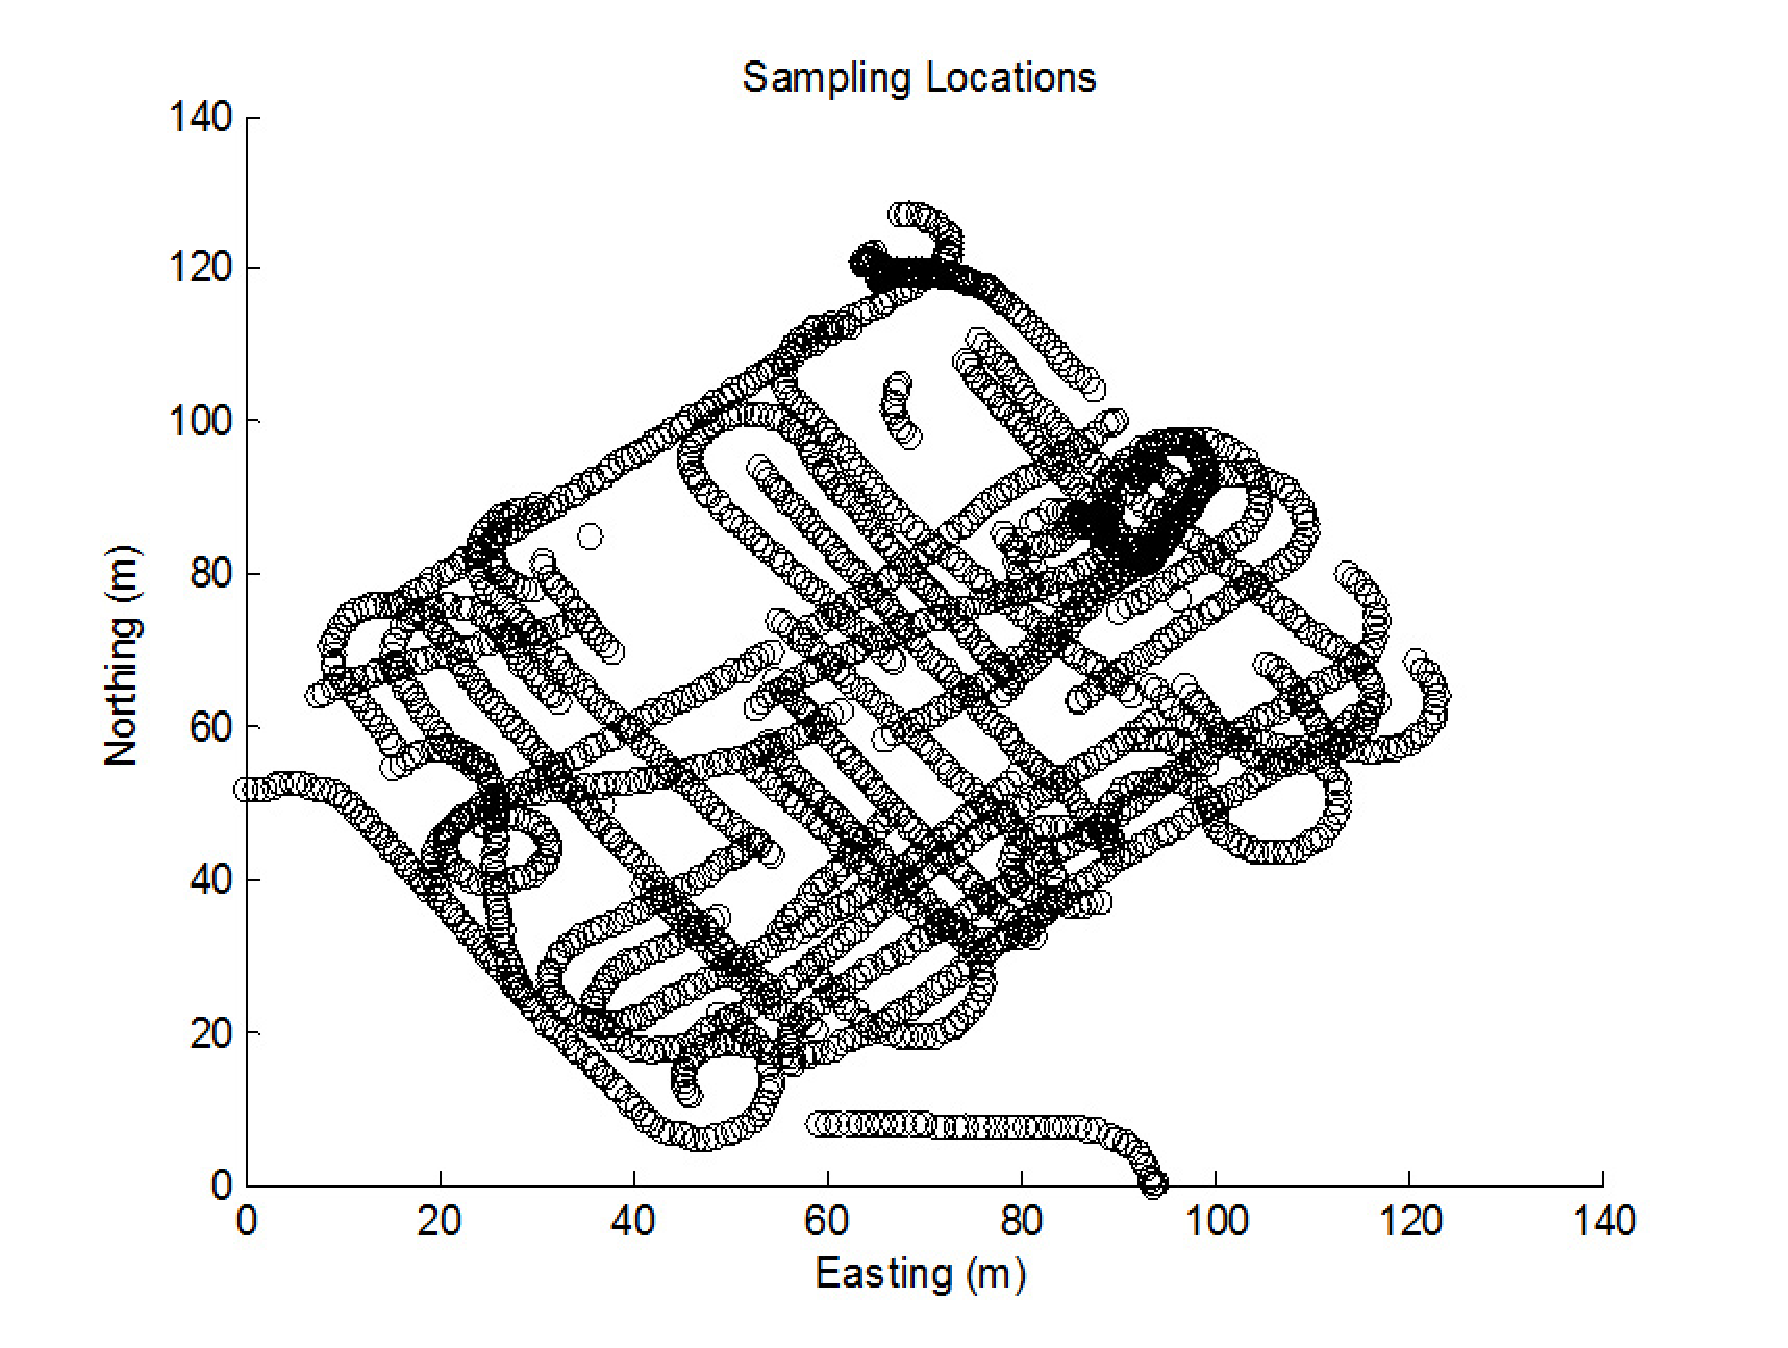
\includegraphics[width=\columnwidth, scale= 0.25]{figs/samplingLocations}
	\caption{Representation of the Sampling Locations.}
	\end{subfigure}
	
	\vspace{0.5cm}
	
	\begin{subfigure}[t]{0.35\textwidth}
	\centering
		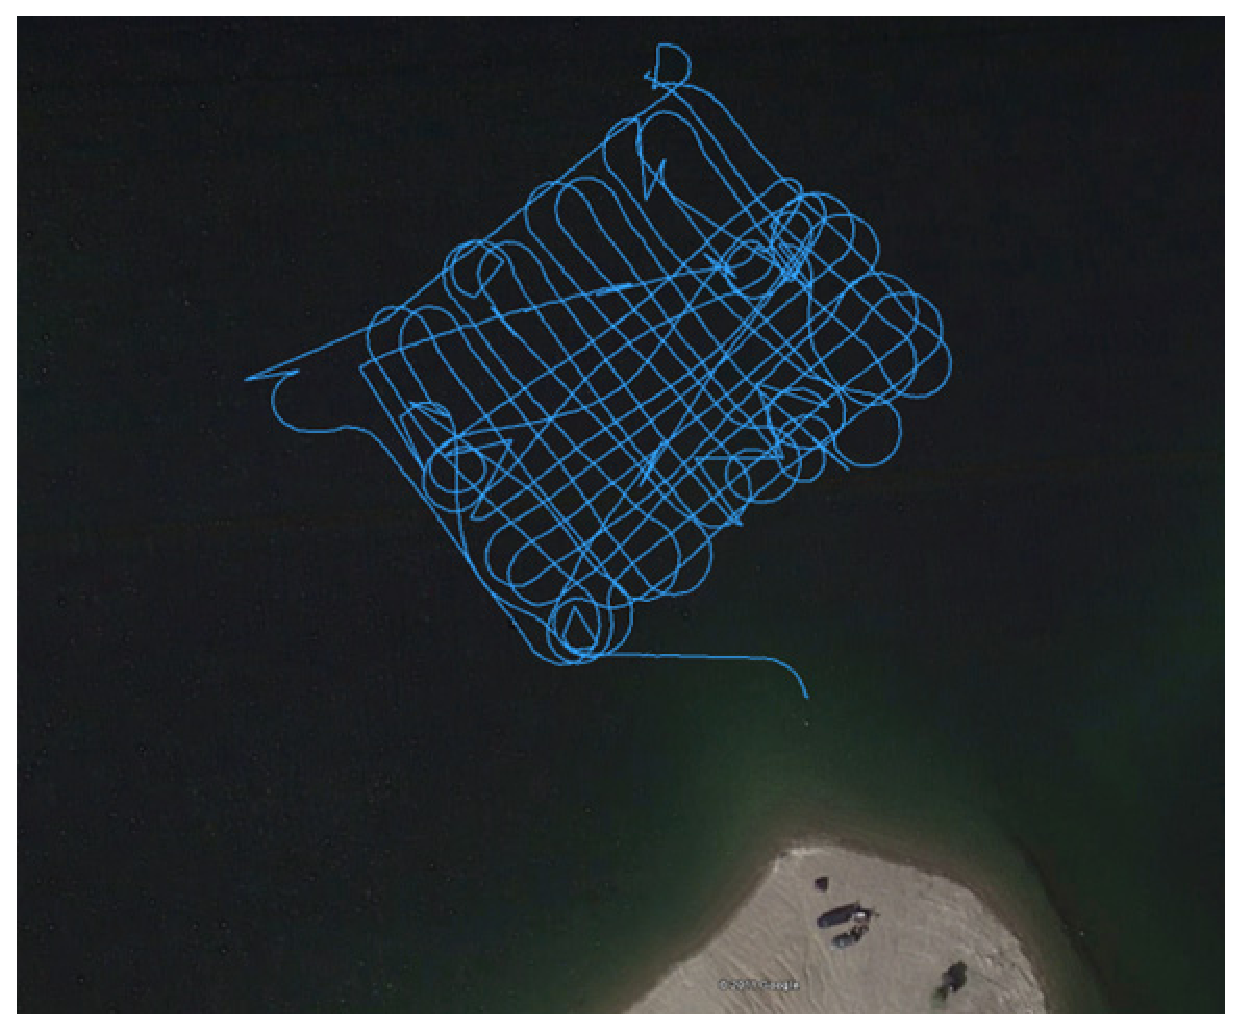
\includegraphics[width=\columnwidth, scale= 0.25]{figs/samplingOverGoogleEarth}
	\caption{Sampling Path at Lake Pleasant.}
	\end{subfigure}
	\caption{Sampling pattern performed during field deployments.}
	\label{fig:fieldDeployments}
\end{figure}

%%%%%%%%%%%%%%%%%%%%%%%%%%%%%%%%%%%%%%%%%%%%%%%%%%%%%%%%%%%%%%%%
\section{Experimental Sampling Path Strategies}
Planning schemes require a priori knowledge of the environment or real time sensing and data feedback. 
There are many AUV deployments scenarios where there is a lack of a priori data on the environment, and the AUV is equipped with sensors that do not provide real time data (such as taking physical water samples) \citep{stoker:exploration}. 
Therefore, in many real world deployments, the paths chosen are often simple lawnmower patterns that may or may not be optimal for the situation they are being utilized \citep{forrest:investigation}, \citep{stoker:exploration}. 
The evaluation conducted in this paper is targeted at looking at autonomous underwater vehicle path planning from an experimental field scientist�s data sampling perspective. 
The goal is to comparatively evaluate various sampling path strategies using a cost-evaluation function that can optimize multiple parameters. 
These results from this evaluation will aid choosing the best sampling path strategy for unknown scalar fields, with no real time data feedback.

\begin{figure*}[t]
	\begin{subfigure}[t]{\columnwidth}
    	\centering
        \includegraphics[scale= 0.30]{figs/lawn_path_evenPlot} 
        \caption{Even lawn mown}
        \label{fig:lawn_path_evenPlot}
     \end{subfigure}
     ~
     \begin{subfigure}[t]{\columnwidth}
    	\centering
        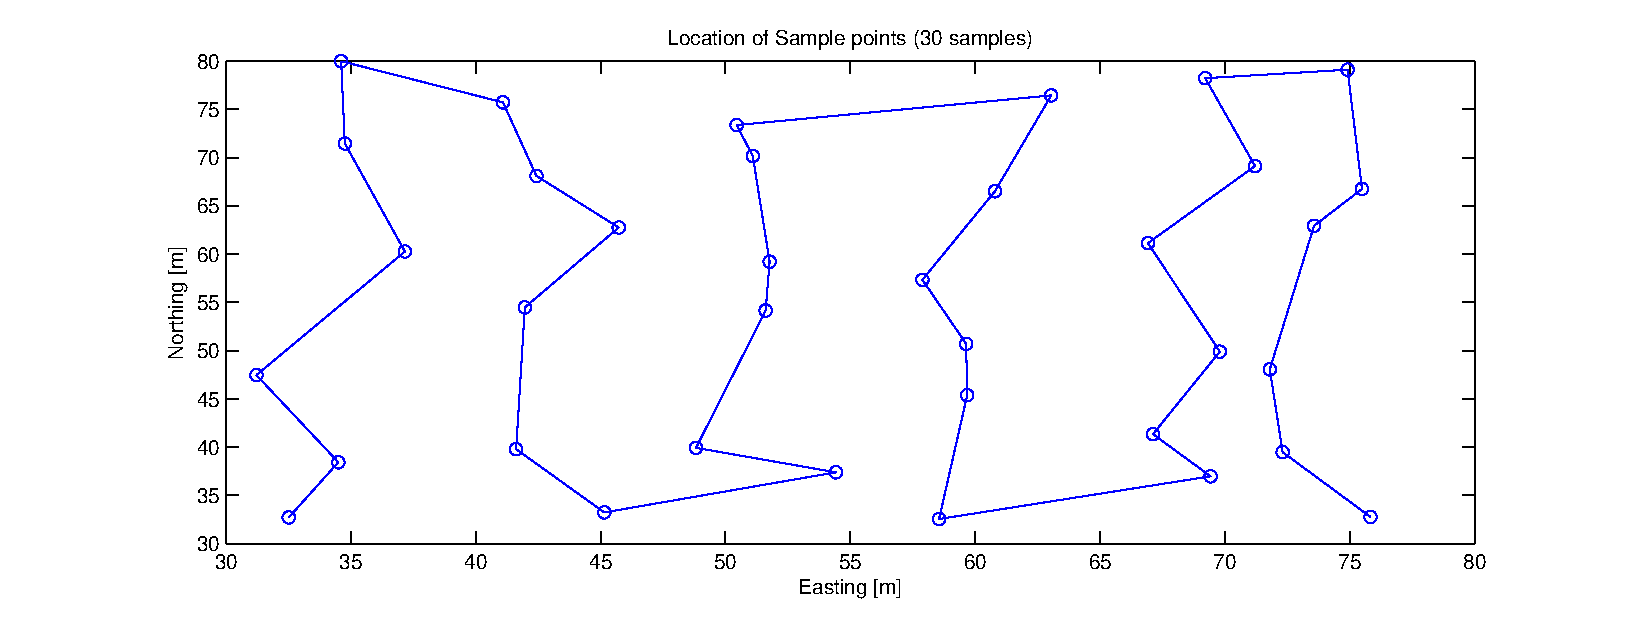
\includegraphics[scale= 0.30]{figs/lawn_pathPlot}
        \caption{Random lawn mown}
        \label{fig:lawn_pathPlot}
     \end{subfigure}

    \begin{subfigure}[b]{\columnwidth}
    	\centering
        \includegraphics[scale= 0.30]{figs/Spiral_path_evenv2Plot}
        \caption{Even spiral}
        \label{fig:Spiral_path_evenv2Plot}
     \end{subfigure}
     ~
     \begin{subfigure}[b]{\columnwidth}
    	\centering
        \includegraphics[scale= 0.30]{figs/Spiral_path_v2Plot}
        \caption{Random spiral}
        \label{fig:Spiral_path_v2Plot}
     \end{subfigure}
 \caption{Examples of the four evaluated sampling patterns}
 \label{fig:samplingPatterns}
\end{figure*}

\subsection{Experimental Approach}
The evaluation consisted of conducting AUV sampling paths over various scalar fields to generate estimations of those scalar fields, and the energy consumption of the sampling path taken. 
Each of the simulated sampling paths and their corresponding scalar field estimation and energy consumption are then used as inputs for a cost-evaluation function that is used to comparatively determine the optimal sampling path.

\subsection{Assumptions}
\label{subsec:initAssump} 
The following assumptions are made:
\begin{itemize}
    \item[1)] The simulated AUV travels at a constant velocity and is capable of navigating to the desired sampling locations.
    \item[2)] The vehicle�s total energy consumption is based upon the total distance it travels, and the total angle it turns.
    \item[3)] The underlying scalar field being sampled has little or no temporal variation while being sampled.
    \item[4)] There is no real-time access to the sampled data; the samples can only be accessed offline.
 \end{itemize}
  
\subsection{Sampling Strategies}
The two main sampling strategy types that are evaluated are systematic sampling, and stratified random sampling.  
Systematic sampling is defined as sampling from an area of interest at regularly spaced intervals. 
Prior research has shown that having equilateral sampling grids is only optimal when the scalar field variation is isotropic \citep{mcbratney:exploration}. 
Therefore stratified random sampling was chosen as an additional sampling method to be comparatively evaluated. 
Stratified random sampling is conducted by splitting the desired sampling area into grid of equal sized sub-areas, in which samples are chosen from a random location in each sub-area. 
Stratified random sampling often produces a weighted mean with less variability than a standard random sampling. 
For each type of sampling strategy, lawn mower and spiral path patterns are evaluated. 
Both are simple path patterns which are commonly used for surveying. 
Example paths of the four sampling strategies are shown in Figure \ref{fig:samplingPatterns}.

\subsection{Underlying Scalar Field Data}
The underlying scalar field was represented with both real world and simulated data. 
The goal was to utilize enough scalar field data to be representative of many scalar field distributions commonly seen in real world data sets. 
Thus, six different underlying scalar fields were generated and collected for the purposes of this evaluation and are shown in Figure \ref{fig:underScalarFields}. 
The data sets derived from real world data consisted of a turbidity data set representing multi-modal data, a chlorophyll data set representing high anisotropy and variance, and a blue green algae cell count data set representing moderate anisotropy data with a high degree of spatial variance. 
The first simulated data set was a linearly varying distribution representing isotropic data. 
The second simulated data set was a normal distribution that represented moderately anisotropic data. 
The third and final simulated data set was a bi-modal normal distribution that represented moderate-variance anisotropic data.

\begin{figure*}[t]
	\begin{subfigure}[t]{0.3\textwidth}
    	\centering
        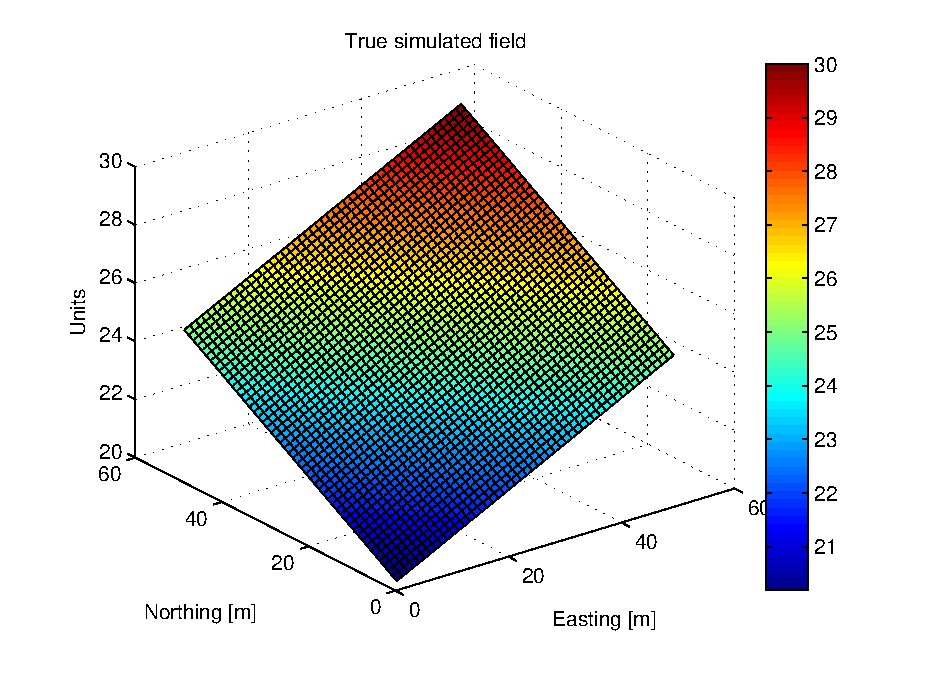
\includegraphics[scale= 0.30]{figs/Isotropic_spiral_even_8x7_true} %width=\columnwidth, scale= 1.0
        \caption{Isotropic}
        \label{fig:Isotropic_spiral_even_8x7_true}
     \end{subfigure}
     ~
     \begin{subfigure}[t]{0.3\textwidth}
    	\centering
        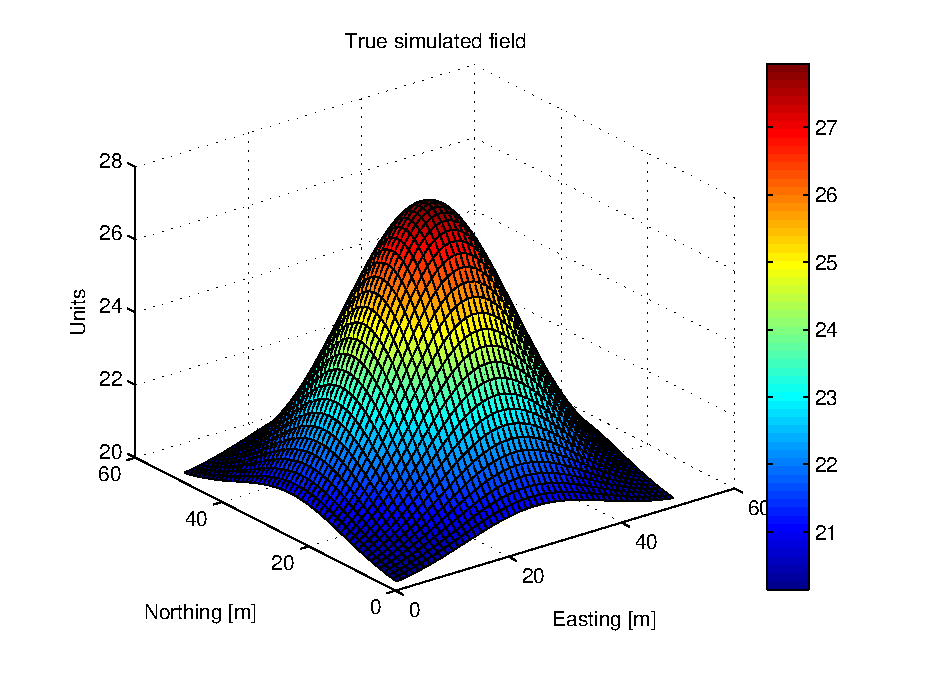
\includegraphics[scale= 0.30]{figs/Anisotropic1_spiral_even_8x7_true}
        \caption{Anisotropic 1}
        \label{fig:Anisotropic1_spiral_even_8x7_true}
     \end{subfigure}
     ~
	\begin{subfigure}[t]{0.3\textwidth}
    	\centering
        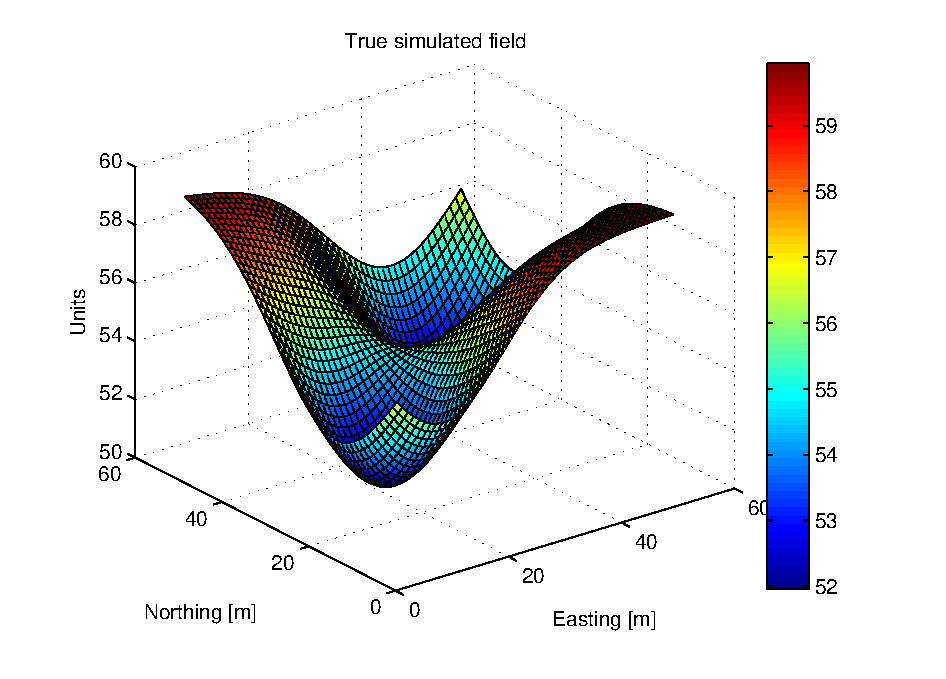
\includegraphics[scale= 0.30]{figs/Anisotropic4_spiral_even_12x10_true}
        \caption{Anisotropic 2}
        \label{fig:Anisotropic4_spiral_even_12x10_true}
     \end{subfigure}
     
     \vspace{0.5cm}
     
     \begin{subfigure}[b]{0.3\textwidth}
    	\centering
        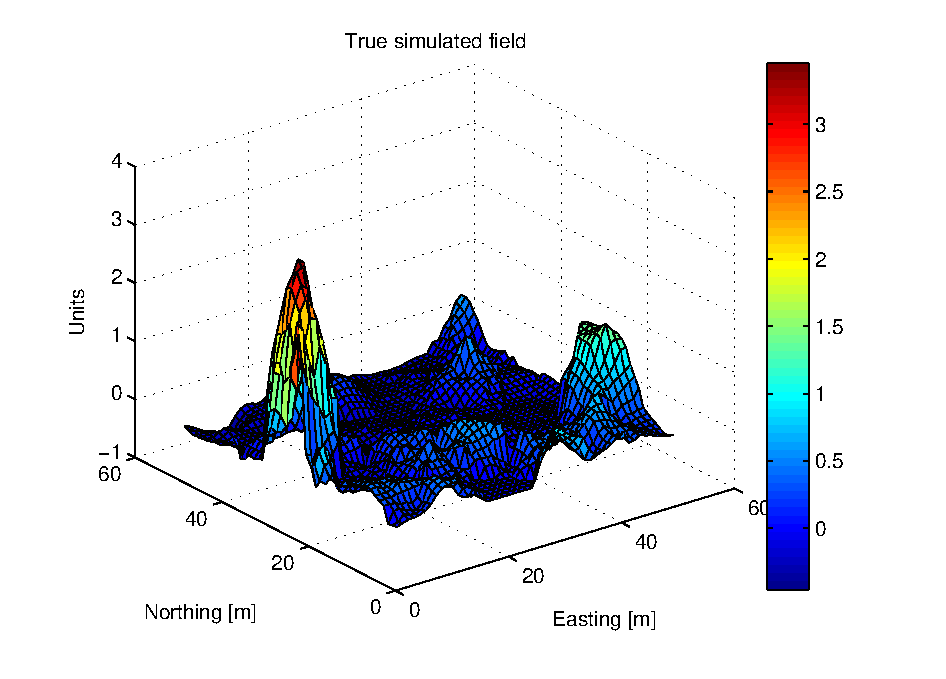
\includegraphics[scale= 0.30]{figs/Turbidity_spiral_even_10x9_true}
        \caption{Turbidity}
        \label{fig:Turbidity_spiral_even_10x9_true}
     \end{subfigure}
	 ~
     \begin{subfigure}[b]{0.3\textwidth}
    	\centering
        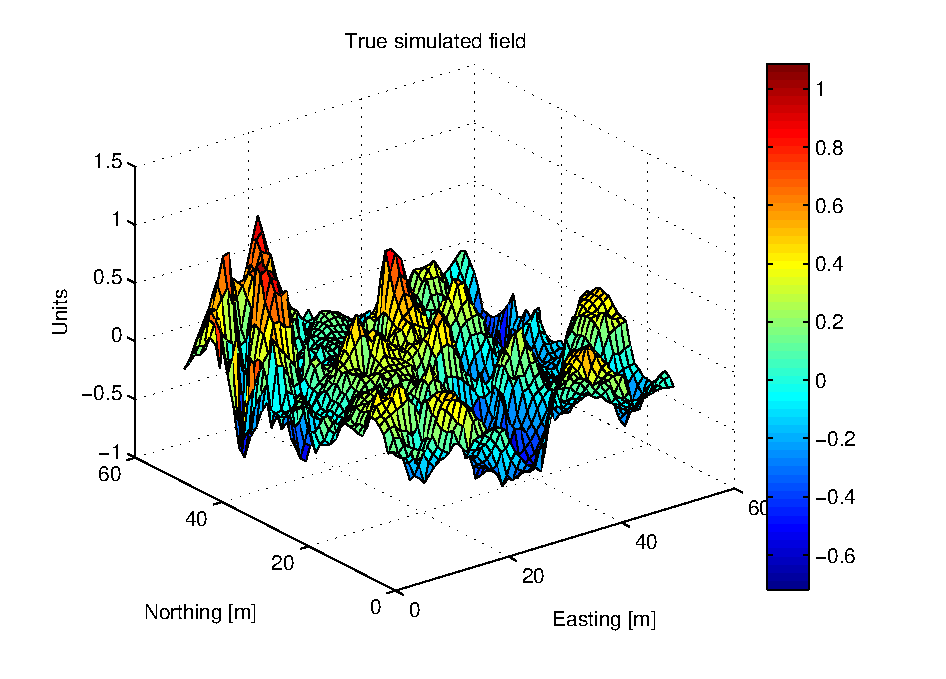
\includegraphics[scale= 0.30]{figs/Cholorophyll_spiral_rand_9x8_true}
        \caption{Cholorophyll}
        \label{fig:Cholorophyll_spiral_rand_9x8_true}
     \end{subfigure}
     ~
     \begin{subfigure}[b]{0.3\textwidth}
    	\centering
        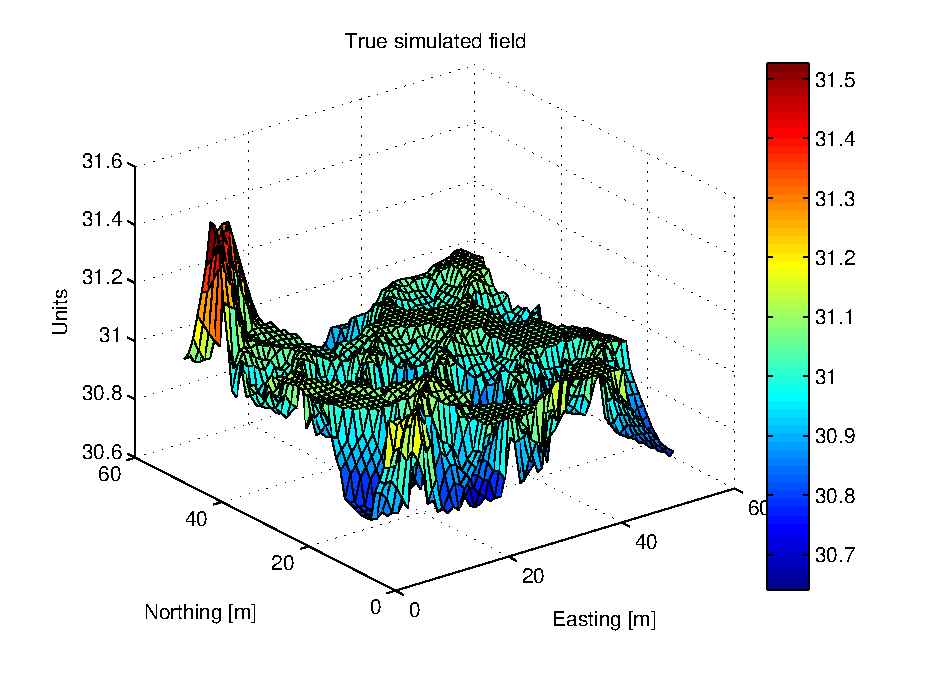
\includegraphics[scale= 0.30]{figs/BlueGreenAlgae_lawn_rand_12x10_true}
        \caption{Blue Green Algae}
        \label{fig:BlueGreenAlgae_lawn_rand_12x10_true}
     \end{subfigure}
 \caption{Examples of the four evaluated sampling patterns}
 \label{fig:underScalarFields}
\end{figure*}


%%%%%%%%%%%%%%%%%%%%%%%%%%%%%%%%%%%%%%%%%%%%%%%%%%%%%%%%%%%
\section{Evaluation Methods}

\subsection{Estimation Evaluation}
Once a sampling path has been generated, it is then used to sample the underlying scalar field. 
With those samples, an estimation of the underlying scalar field is generated through ordinary Kriging. 
Kriging is a form of linear least squares estimation that interpolates the value of a location upon a scalar field from known values at nearby locations, which in this case are the sampled locations \citep{delhomme:kriging}.
Ordinary Kriging \citep{chiles:ordKrig} is a type of Kriging that assumes that the experimental variogram can be constructed, and that the mean of the scalar field being estimated is unknown but constant. 
$z(x)$ represents the underlying scalar field, thus the Kriging estimation of the scalar field at any location is the weighted average of observed values. 
This is represented through the following equation (\ref{eq:scalarField}). 

\begin{equation}
z(x_0) = \Sigma^n_{i=1} w_i z(x_i)
\label{eq:scalarField}
\end{equation}

The estimation variance of $z(x_0)$ is given by

\begin{equation}
\sigma^2_k = 2 \Sigma^n_{i=1} w_i \gamma(x_i, x_0) - \Sigma^n_{j=1} w_i w_j \gamma(x_i, x_j)
\label{eq:estimVar}
\end{equation}

where $\gamma(x_i, x_0)$ is the variogram of $x_i$ and $x_0$. 
The weights $w_i(x)$ are chosen such that they sum to fulfill the unbiasedness condition (they all sum to $1$), and also minimize the estimation variance.
Thus, the weights are determined through the equation (\ref{eq:weights})

\begin{equation}
\Sigma^n_{j=1} w_j \gamma(x_i, x_j) + \psi = \gamma(x_i, x_0)
\label{eq:weights}
\end{equation}

where $\psi$ is the Lagrance parameter associated with the minimization.
Once the Kriging estimation was generated, it accuracy is evaluated through the computation of its integrated mean square error (IMSE) with respect to the underlying scalar field.


\subsection{Energy Consumption Evaluation}

\subsubsection{Simple Approach}
\label{subsubsection:simpleApprach}
The energy consumed by the vehicle travelling along the sampling path was computed through the use of a simple energy consumption model.
The model has two input parameters; the distance travelled, and the total angle turned.
Since it is assumed that the vehicle is travelling straight at a constant velocity, it is extrapolated that the vehicle consumes its stored energy at a constant rate.
An autonomous underwater vehicle may also experience in increase in energy consumption while turning.
This additional increase may be nominal or significant, depending on the design of the vehicle.
Therefore the model takes the additional energy consumption while turning into consideration through the use of a constant multiplier for the total turn angle.
The energy consumption equation is modeled through the following equation \ref{eq:energyConsumption}:

\begin{equation}
E(d, \theta) = d + k_\theta
\label{eq:energyConsumption}
\end{equation}

For this equation, $d$ and $\theta$ respectively represent the total distance of the sampling path, and the cumulative turn angle.
The constant $k_\theta$ is a constant multiplier that represents the increase in energy consumption while turning for a vehicle.
This weight is better understood through the following relationship,

\begin{equation}
k_\theta = \frac{d_t}{90^o}
\label{eq:weightK}
\end{equation}

This relation defined as such; for each right angle turn taken, an additional energy penalty of travelling a straight distance $d_t$ is added.

\subsubsection{Dynamic Modeling Approach}
Mobile robotics are key to facilitate and improve the automation of environmental sensing, however the length they can cover is limited by the amount of energy they carry with them.
In our experimental setting, the problem then depends on how the sampling patterns studied in this paper affect the amount of stored energy our platform holds onboard.
Using the simple model approach presented in Section \ref{subsubsection:simpleApprach} as a starting point, we would like to argue for the feasibility of a new approach to model the dynamic behavior of the AUV used in this research: dynamic modelling. 

Although solving the kinematics and dynamics of a mobile robot and in this particular case of a torpedo-like AUV is a well understood task, its solution is highly dependent on parameters such as its physical dimensions and forces acting on the robot.
It is also time-consuming as it usually deals with large matrices and its computation is complex.
This approach may simplify this procedure and to make it easier for non-roboticists to determine the dynamics of their robotic platform based on only the knowledge of the robot's inputs and outputs.

Dynamic modelling consists of an estimation of the dynamical model of the robot based on the selection of two known inputs and one output from the data acquired.
In our particular case, the two inputs of the estimation may be represented by the velocity and the heading of the vehicle measured by the on-board GPS -with a data acquisition frequency set to 2 Hz and the output may be given by the total power consumed by the vehicle during the sampling mission. 

By estimating the dynamical model of the robot, it is not required to assume that the vehicle is travelling straight at a constant velocity, thus there is no restriction with respect to the rate at which the vehicle consumes its stored energy.
An increment in the energy consumed by the vehicle while it turns may be nominal or significant, depending on the design of the vehicle.
The estimated model would then incorporate the possible effect in the increment in energy consumption that a turning maneuver may represent by including the changes in the orientation of the vehicle.

Another advantage of dynamic modelling is that it can be calculated through a wealth of methods.
Two of such methods are the estimation of the state-space model \citep{van:subspace} and an Auto-Regressive eXogeneous (ARX) and Non-Linear ARX model estimator.
Both methods would only require to first estimate the model using the first half of the input data and validate it by using the remaining half of the data set acquired by the vehicle's instruments.

\subsection{Cost-Evaluation Function}
The cost-evaluation function is a general evaluation method that allows for quantitative comparative analysis for multiple input parameters. 
It normalizes and then assigns each input parameter a weight, allowing for the function to prioritize each parameter in respect to one another. 
These weights must all sum to one. 
In the case of this evaluation, we are investigating which sampling strategy is optimal for both estimation error and energy consumption. 
Therefore the parameters that were selected to be inputs for the cost-evaluation function were the total distance travelled  $d$, the total energy consumed $E$, and the IMSE for the specific sampling path taken $\epsilon$.  
Our proposed cost-evaluation function is as follows in equation \ref{eq:costFunction},

\begin{equation}
E(p) = \Sigma_{i=p} W_d N_d d_i + W_E N_E E_i + W_\epsilon N_\epsilon \epsilon_i
\label{eq:costFunction}
\end{equation}

where $W_d$, $W_E$, and $W_\epsilon$, are the weighted factors that provide specific priorities between the total distance travelled, the total energy consumed, and the IMSE for the sampling path taken.  
$N_d$, $N_E$, and $N_\epsilon$ are normalization factors assigned constant values to normalize each of their corresponding parameters and eliminate their dimensions.


%%%%%%%%%%%%%%%%%%%%%%%%%%%%%%%%%%%%%%%%%%%%%%%%%%%%%%%%%%%%%%%%%%%%%%
\section{Experimental Results}
\label{sec:expResults}

\subsection{Underlying Scalar Field Data Generation}
The six different scalar fields used in this evaluation were either generated from simulated equations, or from a real world dataset. 
The isotropic scalar field used for this evaluation was generated by the following equation.

\begin{equation}
I(x, y) = \frac{x+y}{0.1} + 20
\label{eq:isoScalarField}
\end{equation}

The first simulated anisotropic scalar field was generated by using a standard normal distribution and then scaling it by a factor of 50 and offseting by $+20$. 
The multi-modal anisotropic field was generated by simply adding together two equally scaled inverted normal distributions with differing $x-y$ locations for their means. 
The real world dataset used for generating the turbidity, chlorophyll and blue green algae scalar fields was created by sampling a local freshwater lake with an autonomous underwater vehicle carrying a water quality monitoring sonde. 
The contiguous underlying scalar field was then generated by interpolating the samples using ordinary kriging.

\subsection{Estimation Error Computation and Error Result}
To compute the estimation error, an estimate of the underlying scalar field was first generated for each of the sampling strategy types. 
These estimates were generated across varying sampling grid sizes in order to characterize a range of sampling densities from low to high. 
The sampling grid dimensions and total sample size are listed in Table \ref{tab:sampleDistr}.

\begin{table}
\begin{center}
\caption{Sample Distribution Grid Sizes}
\label{tab:sampleDistr}
	\begin{tabular}{|c|c|r|}
		\cline{1-2}
		\multicolumn{2}{|c|}{Grid Dimensions} \\
		\hline
		\it{Size in X} & \it{Size in Y} & \bf{Sample Count}\\
  		\hline
    	5 & 4 & 20 \\
    	\hline
    	6 & 5 & 30 \\
    	\hline
    	7 & 6 & 42 \\
    	\hline
    	8 & 7 & 56 \\
   		\hline
   		9 & 8 & 72 \\
   		\hline
    	10 & 9 & 90 \\
    	\hline
    	12 & 10 & 120 \\
   		\hline
	\end{tabular}
\end{center}
\end{table}

The IMSE for each of the stratified random sampling strategy based estimations was the average of fifteen iterations, in order to generate a stable value. 
The systematic sampling estimation was iterated five times at five separate evenly distributed path seeding locations to remove biasing in error results.
These seeding locations are shown in Figure \ref{fig:pathSeedingPositions}. 

\begin{figure}[htp]
	\centering
		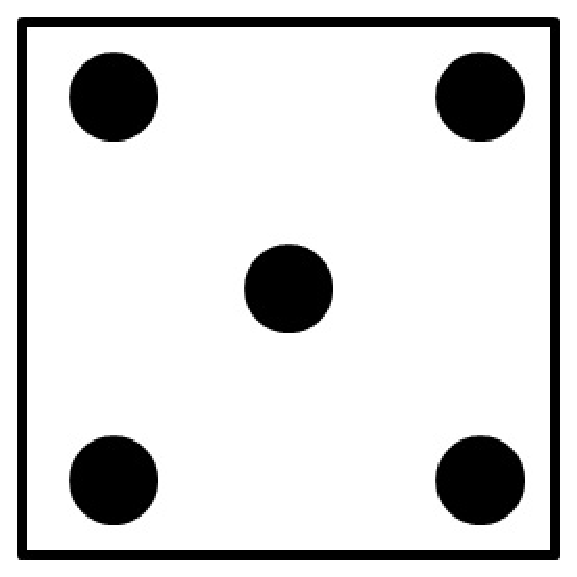
\includegraphics[width=0.10\textwidth]{figs/pathSeedingPositions}
	\caption{Systematic path seeding positions for averaging.}
	\label{fig:pathSeedingPositions}
\end{figure} 

The IMSE error for each of the underlying scalar fields studied are presented in Figure \ref{fig:imseVsDensity}.
From the plot of the IMSE versus number of sample plots for the various underlying scalar fields, a number of correlations are apparent. 
Firstly, both strategies demonstrate a reduction in IMSE as the number of samples increases, as one would expect. 
Additionally, it is found that the systematic sampling strategy minimizes error for the real world data sets across all sampling densities. 
The stratified random sampling strategy minimizes error for the low variance isotropic and anisotropic 2 data sets. 
Finally, for the anisotropic 1 data set, the systematic sampling strategy significantly minimizes error for low sampling densities, and the stratified random sampling strategy minimizes error for moderate and high sampling densities.


\begin{figure*}
	\centering
	\begin{subfigure}[t]{0.35\textwidth}
		\centering
			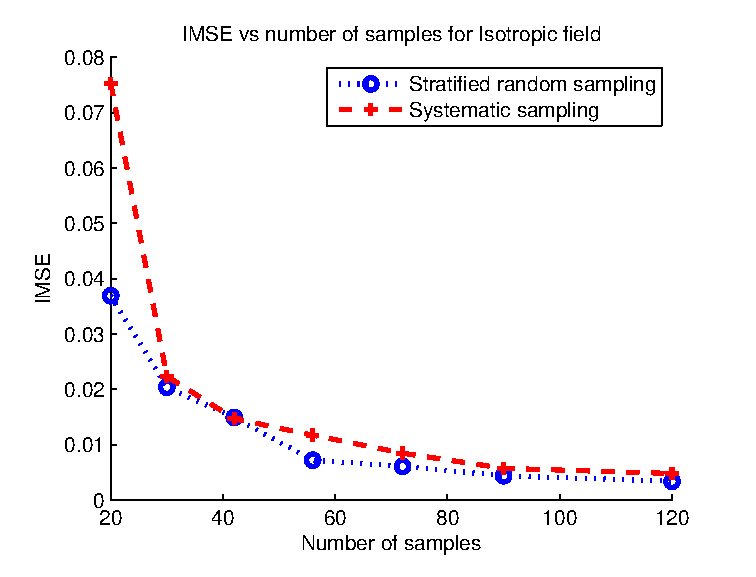
\includegraphics[width=\columnwidth, scale= 0.25]{figs/Isotropic_IMSE}
		\caption{IMSE vs Isotropic scalar field.}
		\label{fig:Isotropic_IMSE}
	\end{subfigure}
	~
	\begin{subfigure}[t]{0.35\textwidth}
		\centering
			\includegraphics[width=\columnwidth, scale= 0.25]{figs/Anisotropic1_IMSE}
		\caption{IMSE vs Anisotropic 1 scalar field.}
		\label{fig:Anisotropic1_IMSE}
	\end{subfigure}
	
	\vspace{0.5cm}
	
	\begin{subfigure}[t]{0.35\textwidth}
		\centering
			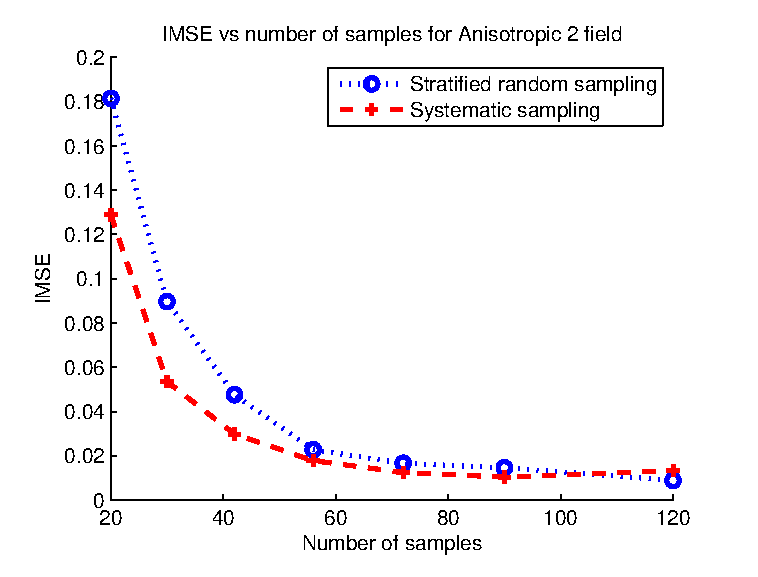
\includegraphics[width=\columnwidth, scale= 0.25]{figs/Anisotropic2_IMSE}
		\caption{IMSE vs Anisotropic 2 scalar field.}
		\label{fig:Anisotropic2_IMSE}
	\end{subfigure}
	~
	\begin{subfigure}[t]{0.35\textwidth}
		\centering
			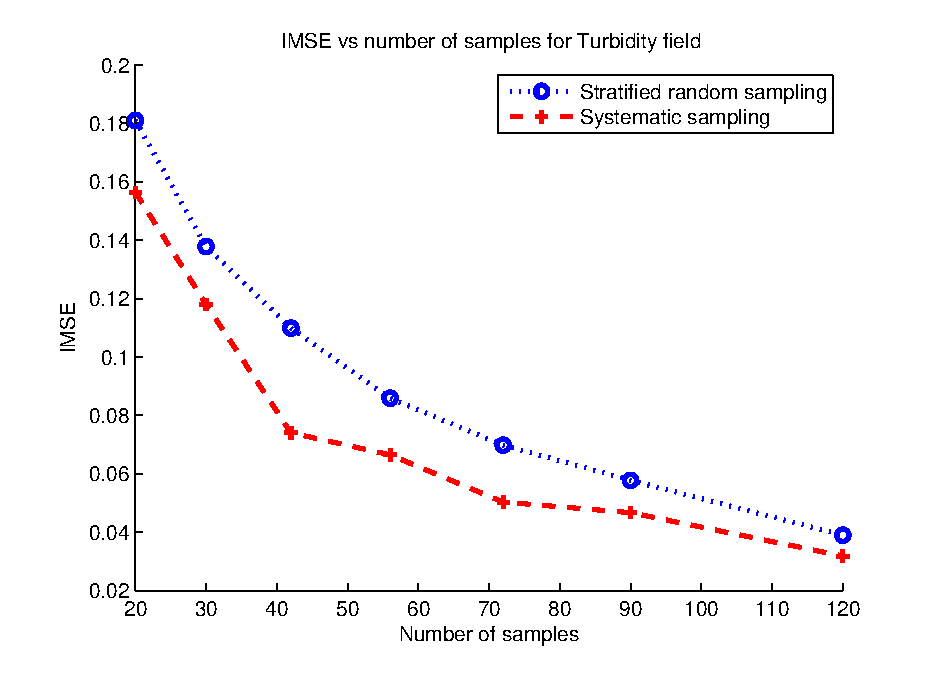
\includegraphics[width=\columnwidth, scale= 0.25]{figs/Turbidity_IMSE}
		\caption{IMSE vs Turbidity scalar field.}
		\label{fig:Turbidity_IMSE}
	\end{subfigure}
	
	\vspace{0.5cm}
	
	\begin{subfigure}[t]{0.35\textwidth}
		\centering
			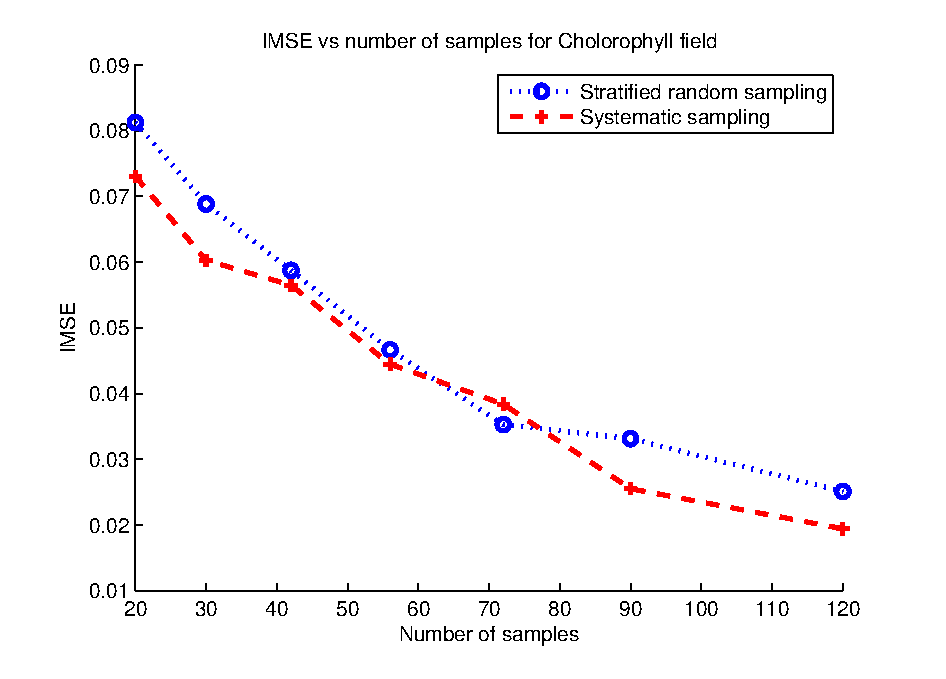
\includegraphics[width=\columnwidth, scale= 0.25]{figs/Cholorophyll_IMSE}
		\caption{IMSE vs Chlorophyll scalar field.}
		\label{fig:Cholorophyll_IMSE}
	\end{subfigure}
	~
	\begin{subfigure}[t]{0.35\textwidth}
		\centering
			\includegraphics[width=\columnwidth, scale= 0.25]{figs/BlueGreenAlgae_IMSE}
		\caption{IMSE vs Blue Green Algae scalar field.}
		\label{fig:BlueGreenAlgae_IMSE}
	\end{subfigure}
	\caption{Integrated Mean-square error estimation for several sample densities across the underlying scalar fields studied.}
	\label{fig:imseVsDensity}
\end{figure*}


\subsection{Energy Consumption Computation and Results} 
The energy consumption of each of the sampling path patterns was computed using equation \ref{eq:energyConsumption}. 
First, the distance and total angle turned was computed for each of the sampling path types through the range of sampling densities shown in Table \ref{tab:sampleDistr}.  
For each of the stratified random sampling paths, the total distance travelled and total cumulative angle turned was computed as the averages of 50 iterations of each sample grid size. 
Finally equation \ref{eq:energyConsumption} was applied using $k_\theta$ values from a range of 0 to 2. 
This range characterizes vehicles for which a $90^o$ turn correlates to consuming the energy equivalent to travelling an additional distance of 0 m to 2 m.

The average total energy consumption versus the $k_\theta$ for each of the sampling path strategies is shown in Figure \ref{fig:avgEnergyCon}. 
The resulting total energy versus $k_\theta$ plots were then fitted to linear equations to quantify their relationship. 
The resulting energy consumption model equations for each of the sampling path strategies are shown summarized below:

\begin{eqnarray}
(Random Lawnmower) 	~~y &=& 162.6x + 1186		\label{eq:randLawn}	\\ 
(Random Spiral)		~~y &=& 162.6x + 1138.1		\label{eq:randSpir}	\\
(Even Lawnmower)	~~y &=& 198.73x + 1097		\label{eq:evenLawn}	\\
(Even Spiral)		~~y &=& 198.73x + 1051.8	\label{eq:evenSpir}
\end{eqnarray}

From equations \ref{eq:randLawn}-\ref{eq:evenSpir} it can be seen that the even spiral strategy -corresponding to Eq. \ref{eq:evenSpir}, is the most energy efficient.
This fact is also apparent from Figure \ref{fig:avgEnergyCon}. 

\begin{figure}[t]
	\centering
	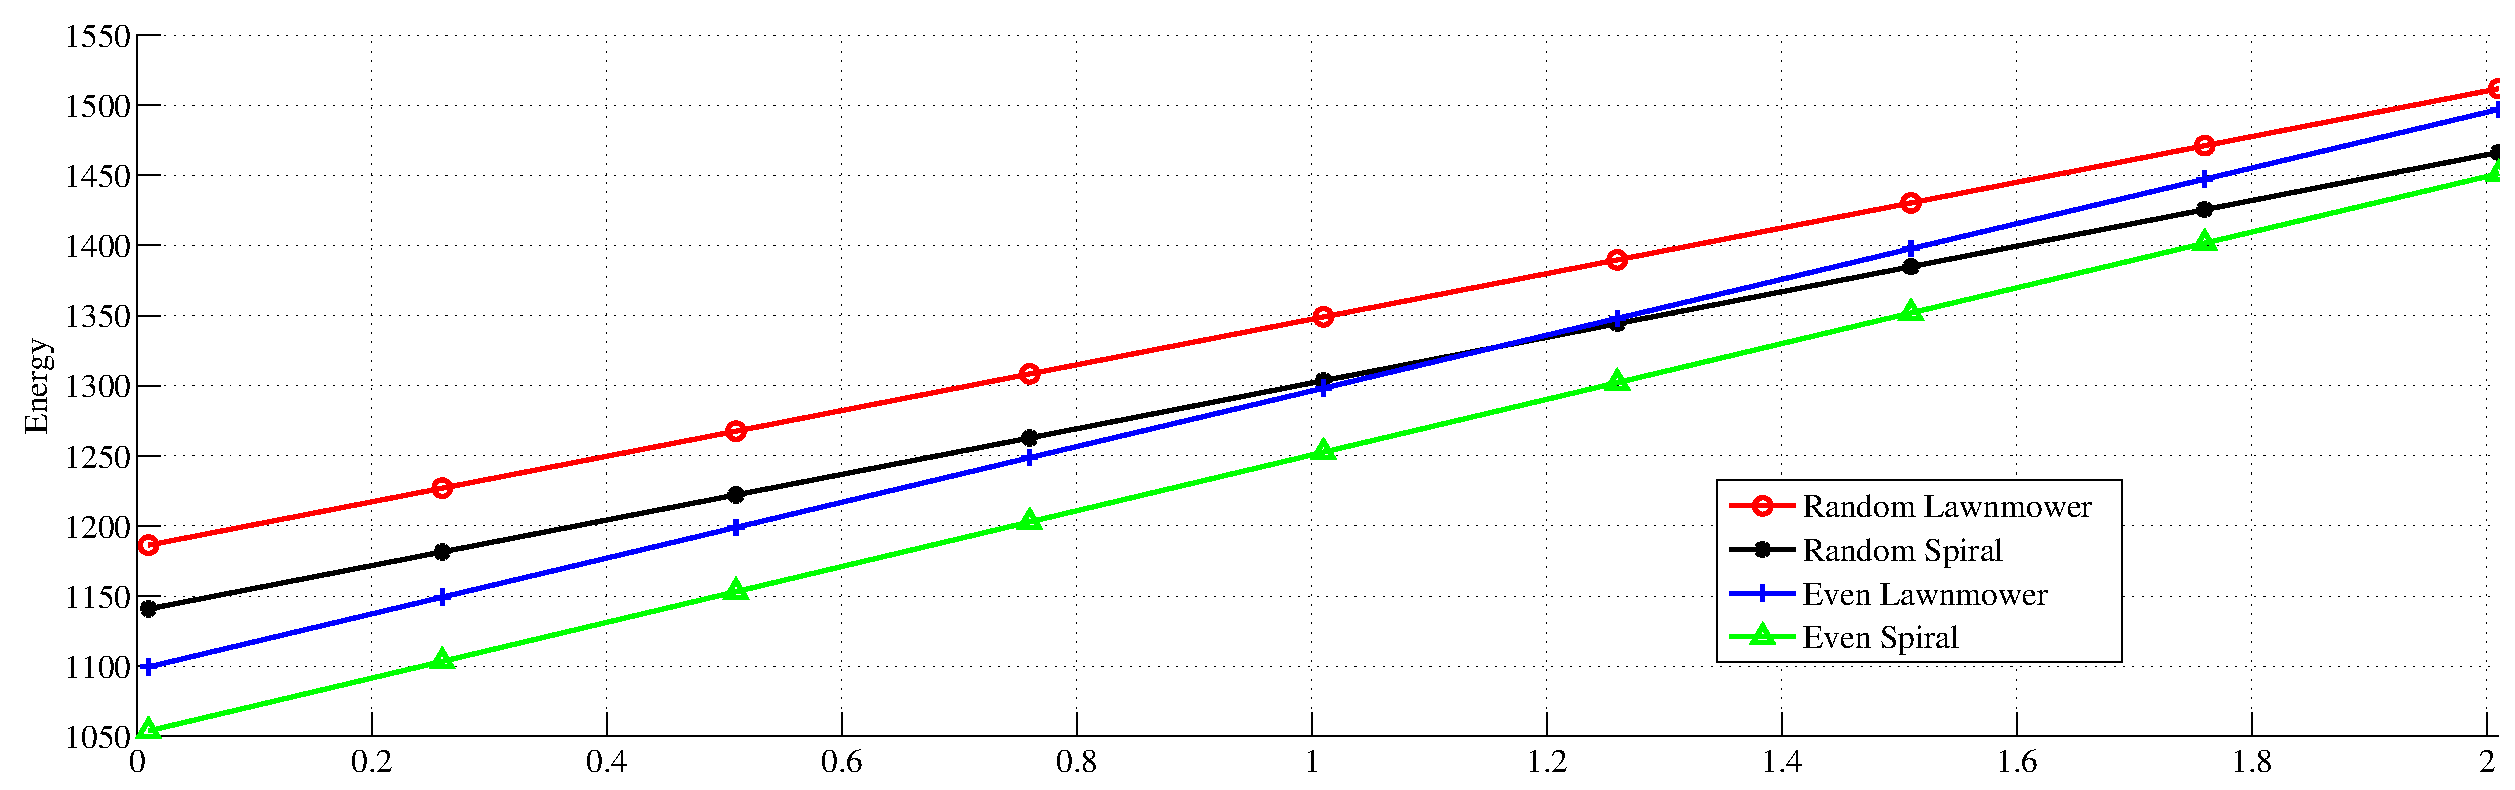
\includegraphics[width=\columnwidth, scale= 0.25]{figs/averageEnergyConsumption}
	\caption{Average energy consumption Vs. $k_\theta$.}
	\label{fig:avgEnergyCon}
\end{figure}

\subsection{Cost-Evaluation Computation and Results}

The cost-evaluation function was computed with the all the weighted factors set equal to $1/3$, thus weighting all of the evaluation parameters equally. 
To compute the energy for each sampling path, $k_\theta$ was set to 0.1. 
The function was applied to each of the sampling strategies for all the underlying scalar fields, at 20, 56, and 120 samples. 
This was done such that a comparative analysis of each of the sampling strategies at low, moderate and high sampling densities could be conducted. 

\begin{figure*}[t]
	\centering
	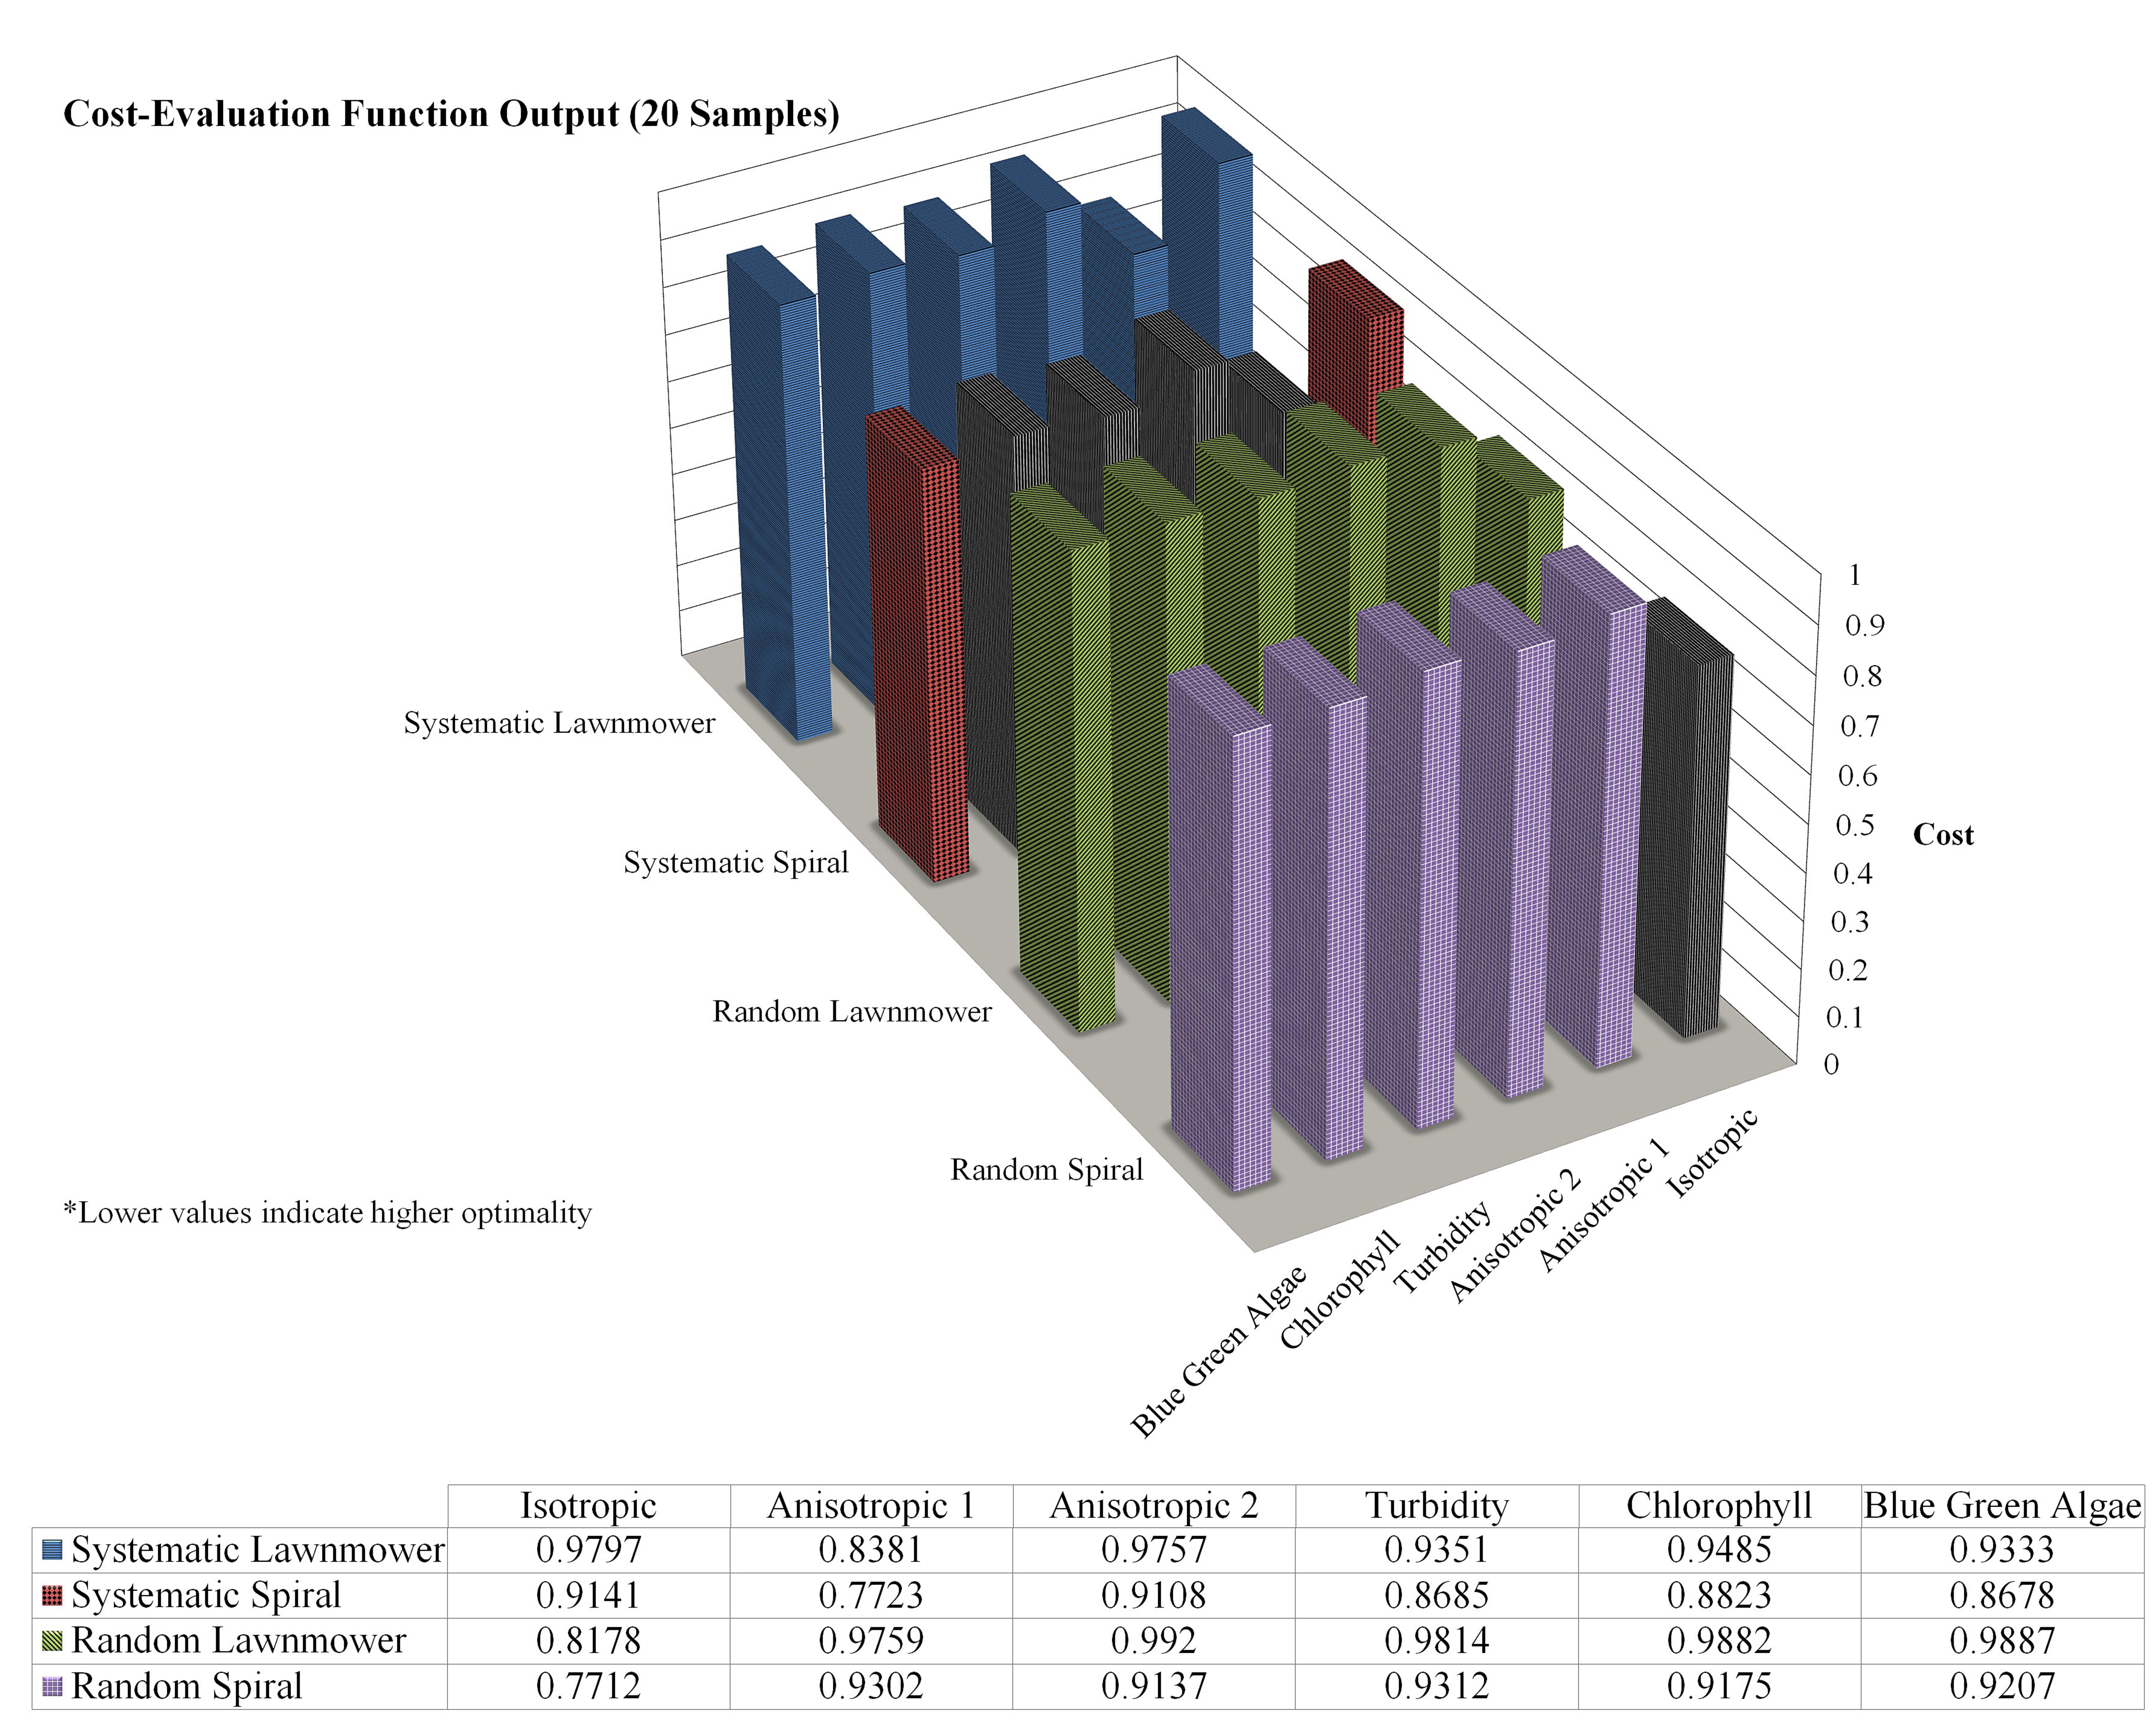
\includegraphics[scale= 0.18]{figs/costEval20Samples} %width=\columnwidth,
	\caption{Cost-evaluation function output for varying scalar fields and sample densities}
	\label{fig:costEvalResults}
\end{figure*}

The results of the cost-evaluation for the 20 samples are listed in Figure \ref{fig:costEvalResults}.
These results reflect a greater cost for higher resulting values, corresponding to less optimality.
The most optimal value is represented by the blocks with black background and white straight lines.
Although the moderate and high sampling densities can be represented in the same manner, we have summarized the results below for the sake of space.

As shown in Figure \ref{fig:costEvalResults}, for the 20 samples density (low sampling density) the systematic spiral sampling method is optimal for all of the data sets (anisotropic 1 0.7723, anisotropic 2 0.9108, turbidity 0.8685, chlorophyll 0.8823, and BGA 0.8678) except for the isotropic scalar field.
In the results of the 56 samples' experiment (moderate sampling density) the systematic lawnmower did not achieve any optimal value, the systematic spiral registered optimal values at the anisotropic 1 (0.7969), turbidity (0.8277), and chlorophyll (0.9188) scalar fields.  
In the results of the 120 samples' experiment (high sampling density) the systematic spiral showed optimality in the turbidity (0.8543), chlorophyll (0.8706), and BGA (0.8689) scalar fields. 
The random spiral indicated optimality for the isotropic (0.8062), anisotropic 1 (0.8331), and the anisotropic 2 (0.8805). 
   
From the experiments above, the strategy that was optimal for the most types of scalar fields and densities was found to be the systematic spiral strategy. 
In general, a spiral path strategy was found to be the optimal in almost all of the cases. 

\section{Discussion}

The approach we present in this papaer can be summarized as follows.
First estimate the underlying scalar field using an ordinary Kriging; then use our proposed energy consumption model and finally determine the most energy-efficient sampling path for an AUV by weighting multiple parameters according to the sampling application. 

The advantages of our approach are the ability to calculate and determine offline which areas would become most representative of the conditions of the body of water being monitored and how to monitor them optimally.
These conditions apply equally to any AUV, independent of its physical characteristics or means of locomotion.
The results of our experiments provide an insight into sampling strategies that are optimal for different types of scalar fields assuming that distance travelled, total energy consumption and IMSE are all equal factors in optimality. 

Our methodology has however, some limitations.
~Although our energy consumption model is a valid model as supported by the results presented, its simplistic nature does not incorportate the effect of forces interacting with the vehicle, the kinematics of the vehicle, the error in its position, or in its velocity control.
Generating an accurate model based on its kinematics and dynamics interaction with a given environment is a task well documented; however, this model is subject to frequent changes since the vehicle is constantly being modified and an accurate representation of the vehicle in all conditions is not feasible.

Dynamic modeling may be a candidate to provide a more straightforward, either simulated-based or data-based energy consumption model of the vehicle. 
This energy consumption model approach allows for a more flexible selection of the data on which the model would be based.
These data are readily available from either previous on-site tests or by simulating the desirable path the vehicle should follow.  
This model provides an accurate relationship between its input or inputs, e.g. velocity and heading, and the output we are focused on: energy consumption.
Dynamic modeling also allows for the modification of the equations that govern the calculation of the model and its outputs.
The authors are currently developing such a model for furter evaluation including a comparative case study with our energy consumption model.


%%%%%%%%%%%%%%%%%%%%%%%%%%%%%%%%%%%%%%%%%%%%%%%%%%%%%%%%%%%%%%
\section{Conclusions}
We presented a straightforward energy consumption model for an AUV sampling a large body of water and a cost-evaluation function that determined the optimal sampling pattern of the AUV across multiple single and multi-modal scalar fields.  

For isotropic scalar fields, the random spiral sampling strategy was found to be the optimal sampling strategy for all sampling densities. 
It was found that in low variance scalar fields, such as the single/multi-modal anisotropic scalar fields used in this evaluation, the systematic spiral strategy is optimal for coarse sampling densities, and the random spiral strategy is optimal for high sampling densities.
In high variance scalar fields such as the turbidity, chlorophyll and blue green algae data sets, the systematic spiral strategy was optimal for almost every case.
In our initial evaluation, we were able to determine that the systematic spiral sampling strategy was the most optimal strategy for minimizing the total path distance, energy consumed, and the IMSE. 
Thus, if one were given the task to choose a sampling strategy given no a priori knowledge of the underlying scalar field and no access to the sampled data in real time, the best sampling strategy to choose would be a systematic spiral path, rather than a standard systematic lawnmower path. 
Through the evaluation, it was demonstrated that the cost-evaluation function is a useful tool that can be used to quantify overall optimality for multiple sampling strategy parameters. 

%\begin{acknowledgements}
%If you'd like to thank anyone, place your comments here
%and remove the percent signs.
%\end{acknowledgements}

% BibTeX users please use one of
\bibliographystyle{plainnat}
%\bibliographystyle{spbasic}      % basic style, author-year citations
%\bibliographystyle{spmpsci}      % mathematics and physical sciences
%\bibliographystyle{spphys}       % APS-like style for physics
\bibliography{autoRobotBib}   % name your BibTeX data base

% Non-BibTeX users please use
%\begin{thebibliography}{}
%
% and use \bibitem to create references. Consult the Instructions
% for authors for reference list style.
%
%\bibitem{RefJ}
% Format for Journal Reference
%Author, Article title, Journal, Volume, page numbers (year)
% Format for books
%\bibitem{RefB}
%Author, Book title, page numbers. Publisher, place (year)
% etc
%\end{thebibliography}

\end{document}
% end of file template.tex

